%%%%%%%%%%%%%%%%%%%%%%%%%%%%%%%%%%%%%%%%%%%%%%%%%
%%%%%%%%%%%%%%%%%%%%%%%%%%%%%%%%%%%%%%%%%%%%%%%%%
\chapter{Results}
\label{chap:results}

In order to evaluate the the algorithms, the analysis of the performance measures from the experiments were organised around three major characteristics of swarm robotics algorithms, namely flexibility, robustness and scalability. Section~\ref{overview} focuses on providing a general overview of algorithm performances, while flexibility of the algorithms over different environmental types and configurations is analysed in Section~\ref{results:flexibility}. Robustness to environmental changes is analysed in Section~\ref{results:robustness}, while Section~\ref{results:scability} does a limited exploration of scalability. Section~\ref{results:summary} summarizes the findings of the experimentation. 

\section{Comparison of Items over Time}
\label{overview}

\begin{table}
\centering
    \caption{Pairwise one-tailed Mann Whitney U wins and losses, averages and standard deviations for the percentage of prioritized items foraged over time, $\sigma$, for each algorithm, over all environments, parameter value choices }
        \label{summarytable}
    \begin{tabular}{l|llll}
    \hline \hline
    Algorithms & Wins & Losses & Average & Std Dev \\ \hline
    Naive      & 1168    & 59042 & 0.528   & 0.394  \\
    Desert Ant  & 42120 & 14557 & 0.643   & 0.387  \\
    Honey Bee   & 45490 & 15179 & 0.807   & 0.294  \\
    \hline
    \end{tabular}
\end{table}

The desert ant, honey-bee and na\"ive foraging algorithms were compared for various robot configurations over different environments, as defined in Chapter~\ref{chap:third}. In order determine whether samples from each experiment came from the same distributions, a Wilcoxin test was performed with $\alpha=0.05$. If the Wilxocin test determines there is a significant difference between the distributions of samples in the two experiments then two one-tailed Mann-Whitney U tests are performed to determine which experiment samples came from a greater distribution, with $\alpha=0.05$. If samples of experiment A is from a greater distribution than the samples of experiment B, then a win is counted for the group of experiments from which experiment A is from and a loss is counted for the group of experiments from which experiment B comes from. 

To understand an algorithms performance against the other algorithms, the wins and losses per each experiment performed for each algorithm, are counted. This statistical analysis approach has been used in \cite{helbig2013performance}. 

Table \ref{summarytable} shows the sum of the wins and losses per algorithm. The pairwise Wilcoxon tests indicate that there exists a significant difference between the results of all three foraging algorithms. Desert ant foraging performed better than na\"ive foraging showing the positive effect of site fidelity. The honey bee algorithm out-performed the na\"ive foraging algorithm and desert ant algorithm indicating the positive effect of communication and adaptivity of the honey bee foraging algorithm. The standard deviation is high for all algorithms due to the extremely large variations in the environments provided. This study rather focuses on a sensitivity study of the algorithms to a variety of environmental, and algorithmic parameters.


\section{Flexibility}
\label{results:flexibility}

In real life environments, it is rarely feasible to optimize parameters per the environment where a swarm of robots needs to be introduced. As a result, it is important that swarm robotics algorithms are insensitive to types of environment and either have a set of parameters that generalize well or have the ability to adapt their parameters to an unseen environment.

To determine the flexibility of the three proposed foraging algorithms, the effect of the ratio of item types in the environment and the effect on different types of distributions of prioritized and non-prioritized items in the environments is analysed. The more insensitive an algorithm is to the change in environmental parameters, the more flexible the algorithm can be considered to be. Section~\ref{results:ratio} analyses the effect of the environmental item ratio on algorithm performance, while the effect of environment type is determined in Section~\ref{results:environmentaltypes}. The effect of item density on algorithm performance is discussed in Section~\ref{results:itemdensity}

\subsection{Environment Item Ratio}
\label{results:ratio}

Environment item ratio, $r$, refers to the ratio of prioritized items to non-prioritized items in a foraging environment. 
Section~\ref{relationship} explores the relationship between environment item ratio and swarm specialization ratio in the performance of na\"ive and desert ant foraging algorithms. The independence of the performance of the honey bee foraging algorithm to environment item ratio is addressed in Section~\ref{Adaptability}.


\begin{table} [h]
    \caption{Effect of environment ratio $r$ on prioritized item foraging per algorithm}
    \label{generalratio}
	\centering
	\footnotesize
	\begin{tabular} {|l|l|l|l|}
		\hline
		Environment Ratio & Na\"ive & Desert Ant & Honey Bee \\
		\hline
		0 & 1 (0)  & 1 (0)  & 1 (0)  \\
		0.2 & 0.339535 (0.376654)  & 0.445135 (0.407285)  & 0.487141 (0.39498)  \\
		0.25 & 0.334883 (0.373433)  & 0.439328 (0.404576)  & 0.477255 (0.393016)  \\
		0.333333 & 0.333027 (0.366004)  & 0.440543 (0.39699)  & 0.478846 (0.384682)  \\
		0.5 & 0.322906 (0.353746)  & 0.433707 (0.386719)  & 0.472925 (0.375211)  \\
		0.666667 & 0.317141 (0.346356)  & 0.428729 (0.380685)  & 0.475938 (0.370087)  \\
		0.75 & 0.313083 (0.342088)  & 0.425262 (0.377452)  & 0.478247 (0.366827)  \\
		0.8 & 0.310814 (0.340525)  & 0.424046 (0.376479)  & 0.480269 (0.365919)  \\
		1 & 0.302589 (0.3297)  & 0.411166 (0.369788)  & 0.493483 (0.360374)  \\
		\hline
	\end{tabular}
\end{table}


\begin{figure}[!htb]
\centering
\resizebox{\textwidth}{!}{% GNUPLOT: LaTeX picture with Postscript
\begingroup
  \makeatletter
  \providecommand\color[2][]{%
    \GenericError{(gnuplot) \space\space\space\@spaces}{%
      Package color not loaded in conjunction with
      terminal option `colourtext'%
    }{See the gnuplot documentation for explanation.%
    }{Either use 'blacktext' in gnuplot or load the package
      color.sty in LaTeX.}%
    \renewcommand\color[2][]{}%
  }%
  \providecommand\includegraphics[2][]{%
    \GenericError{(gnuplot) \space\space\space\@spaces}{%
      Package graphicx or graphics not loaded%
    }{See the gnuplot documentation for explanation.%
    }{The gnuplot epslatex terminal needs graphicx.sty or graphics.sty.}%
    \renewcommand\includegraphics[2][]{}%
  }%
  \providecommand\rotatebox[2]{#2}%
  \@ifundefined{ifGPcolor}{%
    \newif\ifGPcolor
    \GPcolorfalse
  }{}%
  \@ifundefined{ifGPblacktext}{%
    \newif\ifGPblacktext
    \GPblacktexttrue
  }{}%
  % define a \g@addto@macro without @ in the name:
  \let\gplgaddtomacro\g@addto@macro
  % define empty templates for all commands taking text:
  \gdef\gplbacktext{}%
  \gdef\gplfronttext{}%
  \makeatother
  \ifGPblacktext
    % no textcolor at all
    \def\colorrgb#1{}%
    \def\colorgray#1{}%
  \else
    % gray or color?
    \ifGPcolor
      \def\colorrgb#1{\color[rgb]{#1}}%
      \def\colorgray#1{\color[gray]{#1}}%
      \expandafter\def\csname LTw\endcsname{\color{white}}%
      \expandafter\def\csname LTb\endcsname{\color{black}}%
      \expandafter\def\csname LTa\endcsname{\color{black}}%
      \expandafter\def\csname LT0\endcsname{\color[rgb]{1,0,0}}%
      \expandafter\def\csname LT1\endcsname{\color[rgb]{0,1,0}}%
      \expandafter\def\csname LT2\endcsname{\color[rgb]{0,0,1}}%
      \expandafter\def\csname LT3\endcsname{\color[rgb]{1,0,1}}%
      \expandafter\def\csname LT4\endcsname{\color[rgb]{0,1,1}}%
      \expandafter\def\csname LT5\endcsname{\color[rgb]{1,1,0}}%
      \expandafter\def\csname LT6\endcsname{\color[rgb]{0,0,0}}%
      \expandafter\def\csname LT7\endcsname{\color[rgb]{1,0.3,0}}%
      \expandafter\def\csname LT8\endcsname{\color[rgb]{0.5,0.5,0.5}}%
    \else
      % gray
      \def\colorrgb#1{\color{black}}%
      \def\colorgray#1{\color[gray]{#1}}%
      \expandafter\def\csname LTw\endcsname{\color{white}}%
      \expandafter\def\csname LTb\endcsname{\color{black}}%
      \expandafter\def\csname LTa\endcsname{\color{black}}%
      \expandafter\def\csname LT0\endcsname{\color{black}}%
      \expandafter\def\csname LT1\endcsname{\color{black}}%
      \expandafter\def\csname LT2\endcsname{\color{black}}%
      \expandafter\def\csname LT3\endcsname{\color{black}}%
      \expandafter\def\csname LT4\endcsname{\color{black}}%
      \expandafter\def\csname LT5\endcsname{\color{black}}%
      \expandafter\def\csname LT6\endcsname{\color{black}}%
      \expandafter\def\csname LT7\endcsname{\color{black}}%
      \expandafter\def\csname LT8\endcsname{\color{black}}%
    \fi
  \fi
  \setlength{\unitlength}{0.0500bp}%
  \begin{picture}(7200.00,5040.00)%
    \gplgaddtomacro\gplbacktext{%
      \csname LTb\endcsname%
      \put(946,704){\makebox(0,0)[r]{\strut{} 0.3}}%
      \put(946,1229){\makebox(0,0)[r]{\strut{} 0.4}}%
      \put(946,1754){\makebox(0,0)[r]{\strut{} 0.5}}%
      \put(946,2279){\makebox(0,0)[r]{\strut{} 0.6}}%
      \put(946,2804){\makebox(0,0)[r]{\strut{} 0.7}}%
      \put(946,3329){\makebox(0,0)[r]{\strut{} 0.8}}%
      \put(946,3854){\makebox(0,0)[r]{\strut{} 0.9}}%
      \put(946,4379){\makebox(0,0)[r]{\strut{} 1}}%
      \put(1078,484){\makebox(0,0){\strut{} 0}}%
      \put(2223,484){\makebox(0,0){\strut{} 0.2}}%
      \put(3368,484){\makebox(0,0){\strut{} 0.4}}%
      \put(4513,484){\makebox(0,0){\strut{} 0.6}}%
      \put(5658,484){\makebox(0,0){\strut{} 0.8}}%
      \put(6803,484){\makebox(0,0){\strut{} 1}}%
      \put(176,2541){\rotatebox{-270}{\makebox(0,0){\strut{}Prioritized items over time ($\sigma$)}}}%
      \put(3940,154){\makebox(0,0){\strut{}Item Type Ratio ($r$)}}%
      \put(3940,4709){\makebox(0,0){\strut{}Prioritized items over time for each algorithm for item type ratios}}%
    }%
    \gplgaddtomacro\gplfronttext{%
      \csname LTb\endcsname%
      \put(5816,4206){\makebox(0,0)[r]{\strut{}Na\"ive}}%
      \csname LTb\endcsname%
      \put(5816,3986){\makebox(0,0)[r]{\strut{}Desert Ant}}%
      \csname LTb\endcsname%
      \put(5816,3766){\makebox(0,0)[r]{\strut{}Honey Bee}}%
    }%
    \gplbacktext
    \put(0,0){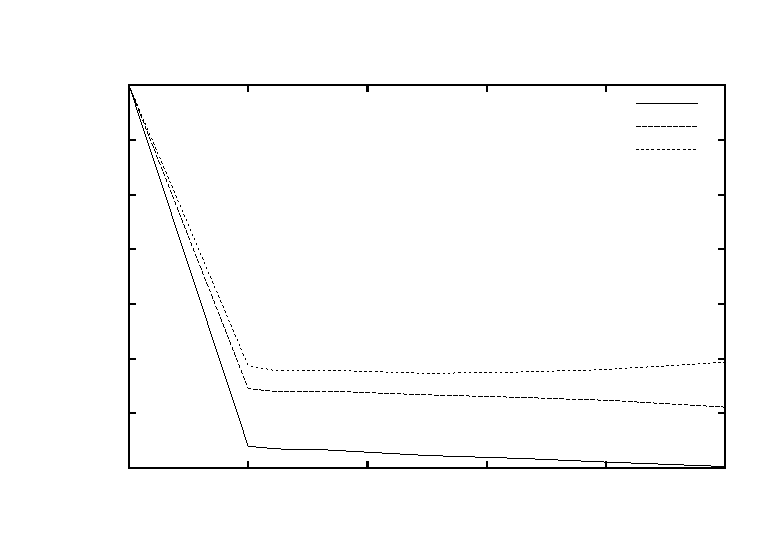
\includegraphics{chapters/chapter6/graphs/gold_ratio}}%
    \gplfronttext
  \end{picture}%
\endgroup
}
\caption{Prioritized items over time over environment ratio $r$ for each algorithm }
\label{ratiogoldplot}
\end{figure}


\begin{figure}[!htb]
\centering
\resizebox{\textwidth}{!}{% GNUPLOT: LaTeX picture with Postscript
\begingroup
  \makeatletter
  \providecommand\color[2][]{%
    \GenericError{(gnuplot) \space\space\space\@spaces}{%
      Package color not loaded in conjunction with
      terminal option `colourtext'%
    }{See the gnuplot documentation for explanation.%
    }{Either use 'blacktext' in gnuplot or load the package
      color.sty in LaTeX.}%
    \renewcommand\color[2][]{}%
  }%
  \providecommand\includegraphics[2][]{%
    \GenericError{(gnuplot) \space\space\space\@spaces}{%
      Package graphicx or graphics not loaded%
    }{See the gnuplot documentation for explanation.%
    }{The gnuplot epslatex terminal needs graphicx.sty or graphics.sty.}%
    \renewcommand\includegraphics[2][]{}%
  }%
  \providecommand\rotatebox[2]{#2}%
  \@ifundefined{ifGPcolor}{%
    \newif\ifGPcolor
    \GPcolorfalse
  }{}%
  \@ifundefined{ifGPblacktext}{%
    \newif\ifGPblacktext
    \GPblacktexttrue
  }{}%
  % define a \g@addto@macro without @ in the name:
  \let\gplgaddtomacro\g@addto@macro
  % define empty templates for all commands taking text:
  \gdef\gplbacktext{}%
  \gdef\gplfronttext{}%
  \makeatother
  \ifGPblacktext
    % no textcolor at all
    \def\colorrgb#1{}%
    \def\colorgray#1{}%
  \else
    % gray or color?
    \ifGPcolor
      \def\colorrgb#1{\color[rgb]{#1}}%
      \def\colorgray#1{\color[gray]{#1}}%
      \expandafter\def\csname LTw\endcsname{\color{white}}%
      \expandafter\def\csname LTb\endcsname{\color{black}}%
      \expandafter\def\csname LTa\endcsname{\color{black}}%
      \expandafter\def\csname LT0\endcsname{\color[rgb]{1,0,0}}%
      \expandafter\def\csname LT1\endcsname{\color[rgb]{0,1,0}}%
      \expandafter\def\csname LT2\endcsname{\color[rgb]{0,0,1}}%
      \expandafter\def\csname LT3\endcsname{\color[rgb]{1,0,1}}%
      \expandafter\def\csname LT4\endcsname{\color[rgb]{0,1,1}}%
      \expandafter\def\csname LT5\endcsname{\color[rgb]{1,1,0}}%
      \expandafter\def\csname LT6\endcsname{\color[rgb]{0,0,0}}%
      \expandafter\def\csname LT7\endcsname{\color[rgb]{1,0.3,0}}%
      \expandafter\def\csname LT8\endcsname{\color[rgb]{0.5,0.5,0.5}}%
    \else
      % gray
      \def\colorrgb#1{\color{black}}%
      \def\colorgray#1{\color[gray]{#1}}%
      \expandafter\def\csname LTw\endcsname{\color{white}}%
      \expandafter\def\csname LTb\endcsname{\color{black}}%
      \expandafter\def\csname LTa\endcsname{\color{black}}%
      \expandafter\def\csname LT0\endcsname{\color{black}}%
      \expandafter\def\csname LT1\endcsname{\color{black}}%
      \expandafter\def\csname LT2\endcsname{\color{black}}%
      \expandafter\def\csname LT3\endcsname{\color{black}}%
      \expandafter\def\csname LT4\endcsname{\color{black}}%
      \expandafter\def\csname LT5\endcsname{\color{black}}%
      \expandafter\def\csname LT6\endcsname{\color{black}}%
      \expandafter\def\csname LT7\endcsname{\color{black}}%
      \expandafter\def\csname LT8\endcsname{\color{black}}%
    \fi
  \fi
  \setlength{\unitlength}{0.0500bp}%
  \begin{picture}(7200.00,5040.00)%
    \gplgaddtomacro\gplbacktext{%
      \csname LTb\endcsname%
      \put(946,704){\makebox(0,0)[r]{\strut{} 0.3}}%
      \put(946,1229){\makebox(0,0)[r]{\strut{} 0.4}}%
      \put(946,1754){\makebox(0,0)[r]{\strut{} 0.5}}%
      \put(946,2279){\makebox(0,0)[r]{\strut{} 0.6}}%
      \put(946,2804){\makebox(0,0)[r]{\strut{} 0.7}}%
      \put(946,3329){\makebox(0,0)[r]{\strut{} 0.8}}%
      \put(946,3854){\makebox(0,0)[r]{\strut{} 0.9}}%
      \put(946,4379){\makebox(0,0)[r]{\strut{} 1}}%
      \put(1078,484){\makebox(0,0){\strut{} 0}}%
      \put(2223,484){\makebox(0,0){\strut{} 0.2}}%
      \put(3368,484){\makebox(0,0){\strut{} 0.4}}%
      \put(4513,484){\makebox(0,0){\strut{} 0.6}}%
      \put(5658,484){\makebox(0,0){\strut{} 0.8}}%
      \put(6803,484){\makebox(0,0){\strut{} 1}}%
      \put(176,2541){\rotatebox{-270}{\makebox(0,0){\strut{}Non-prioritized items over time ($\sigma$)}}}%
      \put(3940,154){\makebox(0,0){\strut{}Item Type Ratio ($r$)}}%
      \put(3940,4709){\makebox(0,0){\strut{}Non-prioritized items over time for each algorithm for item type ratios}}%
    }%
    \gplgaddtomacro\gplfronttext{%
      \csname LTb\endcsname%
      \put(5816,4206){\makebox(0,0)[r]{\strut{}Na\"ive}}%
      \csname LTb\endcsname%
      \put(5816,3986){\makebox(0,0)[r]{\strut{}Desert Ant}}%
      \csname LTb\endcsname%
      \put(5816,3766){\makebox(0,0)[r]{\strut{}Honey Bee}}%
    }%
    \gplbacktext
    \put(0,0){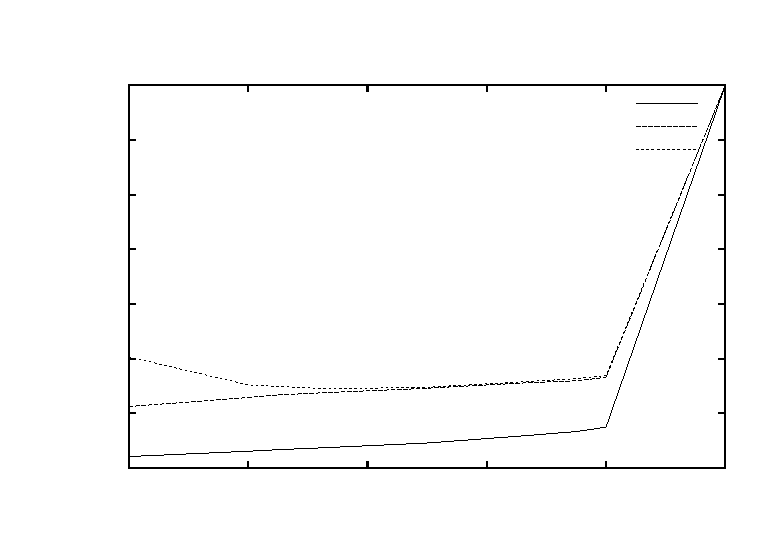
\includegraphics{chapters/chapter6/graphs/waste_ratio}}%
    \gplfronttext
  \end{picture}%
\endgroup
}
\caption{Non-prioritized items over time over environment ratio $r$ for each algorithm}
\label{ratiowasteplot}
\end{figure}


\subsubsection{The Relationship between Environment Item Ratio and Specialization Ratio of Robots}
\label{relationship}
Two hypotheses were formulated and tested. The hypotheses are related to the dependency of the performance of an algorithm in environments of specific environment item ratios and the swarm specialization as follows:

\begin{enumerate}
\item An algorithm that forages a portion of non-prioritized items will have greater performance than an algorithm that does not forage any non-prioritized items.
\item Algorithm performance depends on the environment ratio $r$ and the specialization ratio $\tau$. As $r$ increases, the value of $\tau$ that yields the greatest value of $\sigma$, $\tau_{best}$, will increase approximately linearly for the na\"ive and desert ant algorithms, while the performance of the honey bee algorithm will be independent of $r$ due to division of labour.
\end{enumerate}

An algorithm configured with $\tau=1$ indicates that only prioritized items are foraged. By analysing Table \ref{ratio}, for the na\"ive and desert ant algorithms, for all values of $r$ where $r \neq 1$, $\tau_{best}$ is never equal to $1$, thus the hypothesis that the algorithms achieved the best performance when some robots are configured to forage non-prioritized items is true. The result is likely because non-prioritized items are moved out of the way to allow for easier, faster access to prioritized items or allow access to inaccessible prioritized items.


\begin{table} [h]
     \caption{The performance, $\sigma$, for each foraging algorithm, for each combinations of $r$ and $\tau$. If $\tau_{best}$ exists, $\tau_{best}$ is provided. The best value of $\sigma$ is shown in bold.}
     \label{ratio}
	\centering
	\footnotesize
    \begin{tabular}{|c|c||l|l|l|l|l|l|l|l|l||l|}
	\hline    & & \multicolumn{9}{ |c|| } {$\tau$} &   \\ 
    \cline{3-11}
\multirow{-2}{*}{Algorithm}  &  \multirow{-2}{*}{$r$} & 0     & 0.2   & 0.25  & 0.333 & 0.5   & 0.667  & 0.75  & 0.8    & 1   & \multirow{-2}{*}{$\tau_{best}$ } \\ \hline
    &0     & 1 & 1     & 1     & 1     & 1     & 1     & 1     & 1     & 1     & \\
    &0.2   & 0 & 0.492 & 0.526 & 0.567 & \textbf{0.597} & 0.595 & 0.587 & 0.577 & 0.471 & 0.5 \\
    &0.25  & 0 & 0.484 & 0.526 & 0.557 & 0.588 & \textbf{0.595} & 0.585 & 0.575 & 0.477 & 0.667\\
    &0.333 & 0 & 0.467 & 0.507 & 0.544 & 0.586 & \textbf{0.596} & 0.592 & 0.584 & 0.495 & 0.667\\
    &0.5   & 0 & 0.428 & 0.46  & 0.508 & 0.568 & 0.588 & \textbf{0.591} & 0.589 & 0.528 & 0.75\\
    &0.667 & 0 & 0.4   & 0.433 & 0.487 & 0.544 & 0.583 & \textbf{0.591} & 0.593 & 0.554 & 0.75 \\
    &0.75  & 0 & 0.377 & 0.425 & 0.47  & 0.531 & 0.576 & 0.585 & \textbf{0.591} & 0.567 & 0.8\\
    &0.8   & 0 & 0.372 & 0.409 & 0.455 & 0.53  & 0.571 & 0.584 & \textbf{0.592} & 0.575 & 0.8\\
\multirow{-9}{*}{Na\"ive}&    1     & 0 & 0.336 & 0.375 & 0.433 & 0.5   & 0.552 & 0.57  & 0.581 & \textbf{0.618} & 1\\
     \hline
 &   0                    & 1 & 1     & 1     & 1     & 1     & 1     & 1     & 1     & 1       &    \\
&    0.2                  & 0 & 0.698 & 0.724 & \textbf{0.737} & \textbf{0.737} & 0.712 & 0.694 & 0.67  & 0.519 & 0.333\\
&    0.25                 & 0 & 0.678 & 0.711 & 0.73  & \textbf{0.735} & 0.715 & 0.697 & 0.673 & 0.530 & 0.5 \\
&    0.333                & 0 & 0.65  & 0.693 & 0.722 & \textbf{0.739} & 0.725 & 0.71  & 0.686 & 0.562 & 0.5\\
&    0.5                  & 0 & 0.596 & 0.645 & 0.684 & 0.729 & \textbf{0.734} & 0.725 & 0.701 & 0.621 & 0.667\\
&    0.667                & 0 & 0.554 & 0.607 & 0.648 & 0.706 & 0.737 & \textbf{0.738} & 0.716 & 0.675 & 0.75\\
&    0.75                 & 0 & 0.533 & 0.587 & 0.63  & 0.691 & 0.731 & \textbf{0.739} & 0.72  & 0.703  & 0.75 \\
&    0.8                  & 0 & 0.523 & 0.577 & 0.62  & 0.682 & 0.725 & 0.736 & \textbf{0.74}  & 0.718 & 0.8\\
\multirow{-9}{*}{Desert Ant}&    1                    & 0 & 0.488 & 0.543 & 0.588 & 0.654 & 0.702 & 0.718 & 0.726 & \textbf{0.758} & 1\\ \hline
    %Honey Bee
&        0  & 1     & 1     & 1     & 1     & 1     & 1     & 1     & 1     & 1  &   \\
&    0.2                  & \textbf{0.687} &\textbf{0.687} & 0.686 & 0.686 & 0.686 & 0.685 & 0.686 & 0.685 & \textbf{0.687} &\\
&    0.25                 & 0.678 & \textbf{0.679} & 0.678 & 0.678 &\textbf{0.679} & \textbf{0.679} & 0.678 & 0.677 & \textbf{0.679} &\\
&    0.333                & \textbf{0.674} & \textbf{0.674} & \textbf{0.674} & \textbf{0.674} & \textbf{0.674} & \textbf{0.674} & 0.673 & \textbf{0.674} &\textbf{0.674} &\\
&    0.5                  & 0.668 & \textbf{0.669} & 0.668 & 0.668 & 0.668 & 0.668 & 0.668 & 0.668 & \textbf{0.669} &\\
&    0.667                & 0.671 & 0.671 & 0.671 & 0.671 & 0.671 & \textbf{0.672} & 0.671 & 0.671 & 0.671 &\\
&    0.75                 & 0.672 & \textbf{0.673} & 0.671 & 0.671 & 0.672 &\textbf{0.673} & 0.672 & \textbf{0.673} & \textbf{0.673}&\\
&    0.8                  & 0.674 & 0.674 & 0.674 & 0.674 & 0.674 & \textbf{0.675} &  \textbf{0.675} &  \textbf{0.675} & \textbf{0.675}& \\
\multirow{-9}{*}{Honey Bee}&    1                    & \textbf{0.691} & 0.69  & \textbf{0.691} & 0.69  & \textbf{0.691} &  \textbf{0.691}& 0.69  & 0.69  & 0.69  &\\ \hline

    \end{tabular}

\end{table}

Fig \ref{desertantplot} shows the region in parameter space where the desert ant algorithm performs the best. The na\"ive and desert ant algorithms performed best when $\tau$ was slightly greater than $r$. The existence of the relationship motivates the development of an algorithm that adapts $\tau$ to correspond the environment item ratio $r$.

\begin{figure}[!htb]
\centering
\resizebox{0.8\textwidth}{!}{% GNUPLOT: LaTeX picture with Postscript
\begingroup
  \makeatletter
  \providecommand\color[2][]{%
    \GenericError{(gnuplot) \space\space\space\@spaces}{%
      Package color not loaded in conjunction with
      terminal option `colourtext'%
    }{See the gnuplot documentation for explanation.%
    }{Either use 'blacktext' in gnuplot or load the package
      color.sty in LaTeX.}%
    \renewcommand\color[2][]{}%
  }%
  \providecommand\includegraphics[2][]{%
    \GenericError{(gnuplot) \space\space\space\@spaces}{%
      Package graphicx or graphics not loaded%
    }{See the gnuplot documentation for explanation.%
    }{The gnuplot epslatex terminal needs graphicx.sty or graphics.sty.}%
    \renewcommand\includegraphics[2][]{}%
  }%
  \providecommand\rotatebox[2]{#2}%
  \@ifundefined{ifGPcolor}{%
    \newif\ifGPcolor
    \GPcolorfalse
  }{}%
  \@ifundefined{ifGPblacktext}{%
    \newif\ifGPblacktext
    \GPblacktexttrue
  }{}%
  % define a \g@addto@macro without @ in the name:
  \let\gplgaddtomacro\g@addto@macro
  % define empty templates for all commands taking text:
  \gdef\gplbacktext{}%
  \gdef\gplfronttext{}%
  \makeatother
  \ifGPblacktext
    % no textcolor at all
    \def\colorrgb#1{}%
    \def\colorgray#1{}%
  \else
    % gray or color?
    \ifGPcolor
      \def\colorrgb#1{\color[rgb]{#1}}%
      \def\colorgray#1{\color[gray]{#1}}%
      \expandafter\def\csname LTw\endcsname{\color{white}}%
      \expandafter\def\csname LTb\endcsname{\color{black}}%
      \expandafter\def\csname LTa\endcsname{\color{black}}%
      \expandafter\def\csname LT0\endcsname{\color[rgb]{1,0,0}}%
      \expandafter\def\csname LT1\endcsname{\color[rgb]{0,1,0}}%
      \expandafter\def\csname LT2\endcsname{\color[rgb]{0,0,1}}%
      \expandafter\def\csname LT3\endcsname{\color[rgb]{1,0,1}}%
      \expandafter\def\csname LT4\endcsname{\color[rgb]{0,1,1}}%
      \expandafter\def\csname LT5\endcsname{\color[rgb]{1,1,0}}%
      \expandafter\def\csname LT6\endcsname{\color[rgb]{0,0,0}}%
      \expandafter\def\csname LT7\endcsname{\color[rgb]{1,0.3,0}}%
      \expandafter\def\csname LT8\endcsname{\color[rgb]{0.5,0.5,0.5}}%
    \else
      % gray
      \def\colorrgb#1{\color{black}}%
      \def\colorgray#1{\color[gray]{#1}}%
      \expandafter\def\csname LTw\endcsname{\color{white}}%
      \expandafter\def\csname LTb\endcsname{\color{black}}%
      \expandafter\def\csname LTa\endcsname{\color{black}}%
      \expandafter\def\csname LT0\endcsname{\color{black}}%
      \expandafter\def\csname LT1\endcsname{\color{black}}%
      \expandafter\def\csname LT2\endcsname{\color{black}}%
      \expandafter\def\csname LT3\endcsname{\color{black}}%
      \expandafter\def\csname LT4\endcsname{\color{black}}%
      \expandafter\def\csname LT5\endcsname{\color{black}}%
      \expandafter\def\csname LT6\endcsname{\color{black}}%
      \expandafter\def\csname LT7\endcsname{\color{black}}%
      \expandafter\def\csname LT8\endcsname{\color{black}}%
    \fi
  \fi
  \setlength{\unitlength}{0.0500bp}%
  \begin{picture}(7200.00,5040.00)%
    \gplgaddtomacro\gplbacktext{%
      \csname LTb\endcsname%
      \put(946,704){\makebox(0,0)[r]{\strut{} 0.2}}%
      \put(946,1213){\makebox(0,0)[r]{\strut{} 0.3}}%
      \put(946,1722){\makebox(0,0)[r]{\strut{} 0.4}}%
      \put(946,2231){\makebox(0,0)[r]{\strut{} 0.5}}%
      \put(946,2740){\makebox(0,0)[r]{\strut{} 0.6}}%
      \put(946,3248){\makebox(0,0)[r]{\strut{} 0.7}}%
      \put(946,3757){\makebox(0,0)[r]{\strut{} 0.8}}%
      \put(946,4266){\makebox(0,0)[r]{\strut{} 0.9}}%
      \put(946,4775){\makebox(0,0)[r]{\strut{} 1}}%
      \put(1078,484){\makebox(0,0){\strut{} 0.2}}%
      \put(1794,484){\makebox(0,0){\strut{} 0.3}}%
      \put(2509,484){\makebox(0,0){\strut{} 0.4}}%
      \put(3225,484){\makebox(0,0){\strut{} 0.5}}%
      \put(3940,484){\makebox(0,0){\strut{} 0.6}}%
      \put(4656,484){\makebox(0,0){\strut{} 0.7}}%
      \put(5372,484){\makebox(0,0){\strut{} 0.8}}%
      \put(6087,484){\makebox(0,0){\strut{} 0.9}}%
      \put(6803,484){\makebox(0,0){\strut{} 1}}%
      \put(176,2739){\rotatebox{-270}{\makebox(0,0){\strut{}$\tau$}}}%
      \put(3940,154){\makebox(0,0){\strut{}$r$}}%
    }%
    \gplgaddtomacro\gplfronttext{%
      \csname LTa\endcsname%
      \put(5381,3757){\makebox(0,0)[l]{\strut{}  0.74}}%
      \csname LT0\endcsname%
      \put(5372,4688){\makebox(0,0)[l]{\strut{} 0.72}}%
      \put(6209,3503){\makebox(0,0)[l]{\strut{}  0.72}}%
      \put(1187,958){\makebox(0,0)[l]{\strut{} 0.72}}%
      \csname LT1\endcsname%
      \put(4418,4154){\makebox(0,0)[l]{\strut{} 0.7}}%
      \put(5372,2587){\makebox(0,0)[l]{\strut{}  0.7}}%
      \csname LT2\endcsname%
      \put(4418,4655){\makebox(0,0)[l]{\strut{} 0.68}}%
      \put(5469,2231){\makebox(0,0)[l]{\strut{}  0.68}}%
      \csname LT3\endcsname%
      \put(3225,4277){\makebox(0,0)[l]{\strut{}  0.66}}%
      \put(6201,2307){\makebox(0,0)[l]{\strut{}  0.66}}%
      \csname LT4\endcsname%
      \put(3225,4530){\makebox(0,0)[l]{\strut{}  0.64}}%
      \put(5372,1654){\makebox(0,0)[l]{\strut{}  0.64}}%
      \csname LT5\endcsname%
      \put(2032,4299){\makebox(0,0)[l]{\strut{}  0.62}}%
      \put(5386,1382){\makebox(0,0)[l]{\strut{}  0.62}}%
      \csname LT6\endcsname%
      \put(2032,4462){\makebox(0,0)[l]{\strut{}  0.6}}%
      \put(6267,1382){\makebox(0,0)[l]{\strut{}  0.6}}%
      \csname LT7\endcsname%
      \put(2032,4625){\makebox(0,0)[l]{\strut{}  0.58}}%
      \put(5372,986){\makebox(0,0)[l]{\strut{}   0.58}}%
      \csname LT8\endcsname%
      \put(1436,4564){\makebox(0,0)[l]{\strut{}  0.56}}%
      \put(6087,958){\makebox(0,0)[l]{\strut{}   0.56}}%
      \csname LT0\endcsname%
      \put(1436,4706){\makebox(0,0)[l]{\strut{}  0.54}}%
    }%
    \gplbacktext
    \put(0,0){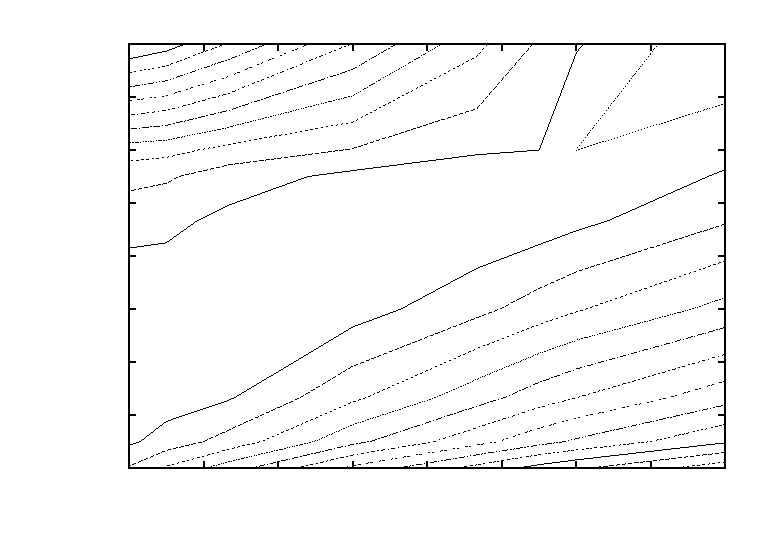
\includegraphics{chapters/chapter6/desertantplot}}%
    \gplfronttext
  \end{picture}%
\endgroup
}
\caption{Contour plot of values for $\sigma$ over values for $r$ and $\tau$ for desert ant foraging}
\label{desertantplot}
\end{figure}


%\begin{figure}
%\input{naiveplot.tex}
%\caption{Contour plot of values for $\sigma$ over values for $r$ and $\tau$ for nai%\"ve foraging}
%\end{figure}

 %But why? Give reason 
%The nai\"ve foraging algorithm slowly clear an entire area around the sink. If there is an equal ratio of robot types to item types then this area would be cleared effectively. 
 %fact that in the more organized environments such as gaussian or vein, it is 

\subsubsection{Independence of the Honey Bee Foraging Algorithm to Item Type Ratio}
\label{Adaptability}

Table~\ref{ratio} indicates that the honey bee foraging algorithm has similar performance throughout all configurations for $r$ and $\tau$, which highlights that the performance of the honey bee algorithm is independent of the value of $\tau$. It can therefore be concluded that, the honey bee algorithm will perform equivalently well, regardless of initial swarm configuration or environmental item ratios, and thus is more flexible.

The desert ant algorithm performed better than the honey bee algorithm, for all values of $r$, when $tau_{best}$ is selected. This indicates that, if the value of $r$ is known for a particular environment, then it is beneficial to use the desert ant foraging algorithm and choose $\tau$ appropriately. A possible reason why the desert ant algorithm performs better when optimally configured for a particular environment than the honey bee algorithm is that the honey bee algorithm takes time to adapt to the environment, while the desert ant algorithm with optimal configurations has no division of labour overhead and may outperform the honey bee algorithm under those circumstances.

\subsection{Environment Item Distributions}
\label{results:environmentaltypes}

\begin{table} [h]
     \caption{Average $\sigma $, the percentage prioritized items over time, for different environment types for each algorithm}
     \label{environmenttypeprioritized}
	\centering
	\footnotesize
	\begin{tabular} {|l|l|l|l|}
\hline
name & Naive & DesertAnt & HoneyBee \\
\hline
clustered & 0.414017 (0.388334)  & 0.504665 (0.396114)  & 0.537091 (0.378332)  \\
gaussian & 0.389998 (0.403603)  & 0.487472 (0.416113)  & 0.542252 (0.399359)  \\
uniform & 0.413511 (0.388773)  & 0.502372 (0.395749)  & 0.530851 (0.376446)  \\
vein & 0.370908 (0.401867)  & 0.482342 (0.419204)  & 0.54274 (0.408115)  \\
\hline
\end{tabular}

\end{table}

\begin{table} [h]
     \caption{Average $\sigma $, the percentage non-prioritized items over time, for different environment types for each algorithm}
     \label{environmenttypenonprioritized}
	\centering
	\footnotesize
	\begin{tabular} {|l|l|l|l|}
\hline
$p$ & Naive & DesertAnt & HoneyBee \\
\hline
5 & 0.620571 (0.375689)  & 0.724854 (0.353456)  & 0.712767 (0.32061)  \\
20 & 0.478558 (0.384724)  & 0.574932 (0.378252)  & 0.586206 (0.369629)  \\
50 & 0.369491 (0.367149)  & 0.451495 (0.379117)  & 0.480418 (0.379408)  \\
70 & 0.327576 (0.356324)  & 0.403477 (0.373719)  & 0.431977 (0.376965)  \\
90 & 0.29737 (0.348107)  & 0.367512 (0.368059)  & 0.39277 (0.37313)  \\
\hline
\end{tabular}

\end{table}

\begin{figure}[!htb]
\centering
\resizebox{0.8\textwidth}{!}{% GNUPLOT: LaTeX picture with Postscript
\begingroup
  \makeatletter
  \providecommand\color[2][]{%
    \GenericError{(gnuplot) \space\space\space\@spaces}{%
      Package color not loaded in conjunction with
      terminal option `colourtext'%
    }{See the gnuplot documentation for explanation.%
    }{Either use 'blacktext' in gnuplot or load the package
      color.sty in LaTeX.}%
    \renewcommand\color[2][]{}%
  }%
  \providecommand\includegraphics[2][]{%
    \GenericError{(gnuplot) \space\space\space\@spaces}{%
      Package graphicx or graphics not loaded%
    }{See the gnuplot documentation for explanation.%
    }{The gnuplot epslatex terminal needs graphicx.sty or graphics.sty.}%
    \renewcommand\includegraphics[2][]{}%
  }%
  \providecommand\rotatebox[2]{#2}%
  \@ifundefined{ifGPcolor}{%
    \newif\ifGPcolor
    \GPcolorfalse
  }{}%
  \@ifundefined{ifGPblacktext}{%
    \newif\ifGPblacktext
    \GPblacktexttrue
  }{}%
  % define a \g@addto@macro without @ in the name:
  \let\gplgaddtomacro\g@addto@macro
  % define empty templates for all commands taking text:
  \gdef\gplbacktext{}%
  \gdef\gplfronttext{}%
  \makeatother
  \ifGPblacktext
    % no textcolor at all
    \def\colorrgb#1{}%
    \def\colorgray#1{}%
  \else
    % gray or color?
    \ifGPcolor
      \def\colorrgb#1{\color[rgb]{#1}}%
      \def\colorgray#1{\color[gray]{#1}}%
      \expandafter\def\csname LTw\endcsname{\color{white}}%
      \expandafter\def\csname LTb\endcsname{\color{black}}%
      \expandafter\def\csname LTa\endcsname{\color{black}}%
      \expandafter\def\csname LT0\endcsname{\color[rgb]{1,0,0}}%
      \expandafter\def\csname LT1\endcsname{\color[rgb]{0,1,0}}%
      \expandafter\def\csname LT2\endcsname{\color[rgb]{0,0,1}}%
      \expandafter\def\csname LT3\endcsname{\color[rgb]{1,0,1}}%
      \expandafter\def\csname LT4\endcsname{\color[rgb]{0,1,1}}%
      \expandafter\def\csname LT5\endcsname{\color[rgb]{1,1,0}}%
      \expandafter\def\csname LT6\endcsname{\color[rgb]{0,0,0}}%
      \expandafter\def\csname LT7\endcsname{\color[rgb]{1,0.3,0}}%
      \expandafter\def\csname LT8\endcsname{\color[rgb]{0.5,0.5,0.5}}%
    \else
      % gray
      \def\colorrgb#1{\color{black}}%
      \def\colorgray#1{\color[gray]{#1}}%
      \expandafter\def\csname LTw\endcsname{\color{white}}%
      \expandafter\def\csname LTb\endcsname{\color{black}}%
      \expandafter\def\csname LTa\endcsname{\color{black}}%
      \expandafter\def\csname LT0\endcsname{\color{black}}%
      \expandafter\def\csname LT1\endcsname{\color{black}}%
      \expandafter\def\csname LT2\endcsname{\color{black}}%
      \expandafter\def\csname LT3\endcsname{\color{black}}%
      \expandafter\def\csname LT4\endcsname{\color{black}}%
      \expandafter\def\csname LT5\endcsname{\color{black}}%
      \expandafter\def\csname LT6\endcsname{\color{black}}%
      \expandafter\def\csname LT7\endcsname{\color{black}}%
      \expandafter\def\csname LT8\endcsname{\color{black}}%
    \fi
  \fi
    \setlength{\unitlength}{0.0500bp}%
    \ifx\gptboxheight\undefined%
      \newlength{\gptboxheight}%
      \newlength{\gptboxwidth}%
      \newsavebox{\gptboxtext}%
    \fi%
    \setlength{\fboxrule}{0.5pt}%
    \setlength{\fboxsep}{1pt}%
\begin{picture}(7200.00,5040.00)%
    \gplgaddtomacro\gplbacktext{%
      \csname LTb\endcsname%
      \put(594,440){\makebox(0,0)[r]{\strut{}$0$}}%
      \put(594,982){\makebox(0,0)[r]{\strut{}$0.1$}}%
      \put(594,1524){\makebox(0,0)[r]{\strut{}$0.2$}}%
      \put(594,2066){\makebox(0,0)[r]{\strut{}$0.3$}}%
      \put(594,2608){\makebox(0,0)[r]{\strut{}$0.4$}}%
      \put(594,3149){\makebox(0,0)[r]{\strut{}$0.5$}}%
      \put(594,3691){\makebox(0,0)[r]{\strut{}$0.6$}}%
      \put(594,4233){\makebox(0,0)[r]{\strut{}$0.7$}}%
      \put(594,4775){\makebox(0,0)[r]{\strut{}$0.8$}}%
      \put(2245,220){\makebox(0,0){\strut{}Na\"ive}}%
      \put(3765,220){\makebox(0,0){\strut{}DesertAnt}}%
      \put(5284,220){\makebox(0,0){\strut{}HoneyBee}}%
    }%
    \gplgaddtomacro\gplfronttext{%
      \csname LTb\endcsname%
      \put(5816,4602){\makebox(0,0)[r]{\strut{}Uniform}}%
      \csname LTb\endcsname%
      \put(5816,4382){\makebox(0,0)[r]{\strut{}Clustered}}%
      \csname LTb\endcsname%
      \put(5816,4162){\makebox(0,0)[r]{\strut{}Gaussian}}%
      \csname LTb\endcsname%
      \put(5816,3942){\makebox(0,0)[r]{\strut{}Vein}}%
    }%
    \gplbacktext
    \put(0,0){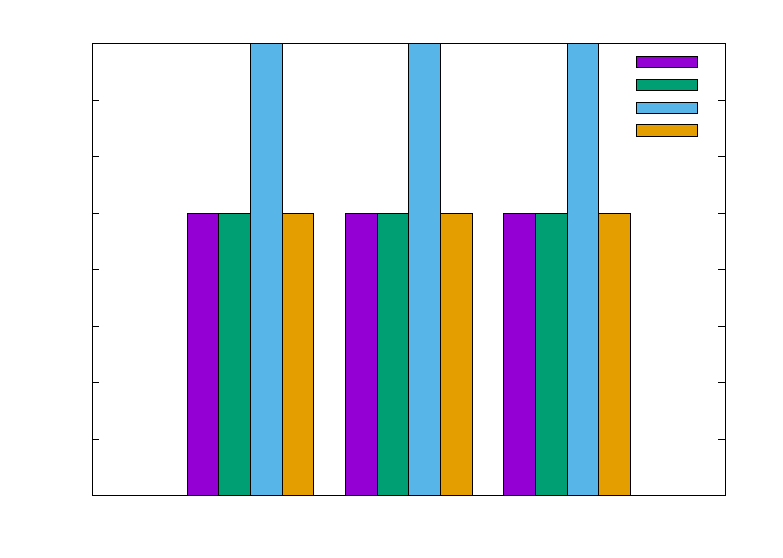
\includegraphics{chapters/chapter6/graphs/environment_types}}%
    \gplfronttext
  \end{picture}%
\endgroup
}
\caption{Average and standard deviation of $\sigma $, the percentage prioritized items over time, for different environment types for each algorithm}
\label{fig:environmenttypes}
\end{figure}


\begin{figure}[!htb]
\centering
\resizebox{0.8\textwidth}{!}{% GNUPLOT: LaTeX picture with Postscript
\begingroup
  \makeatletter
  \providecommand\color[2][]{%
    \GenericError{(gnuplot) \space\space\space\@spaces}{%
      Package color not loaded in conjunction with
      terminal option `colourtext'%
    }{See the gnuplot documentation for explanation.%
    }{Either use 'blacktext' in gnuplot or load the package
      color.sty in LaTeX.}%
    \renewcommand\color[2][]{}%
  }%
  \providecommand\includegraphics[2][]{%
    \GenericError{(gnuplot) \space\space\space\@spaces}{%
      Package graphicx or graphics not loaded%
    }{See the gnuplot documentation for explanation.%
    }{The gnuplot epslatex terminal needs graphicx.sty or graphics.sty.}%
    \renewcommand\includegraphics[2][]{}%
  }%
  \providecommand\rotatebox[2]{#2}%
  \@ifundefined{ifGPcolor}{%
    \newif\ifGPcolor
    \GPcolorfalse
  }{}%
  \@ifundefined{ifGPblacktext}{%
    \newif\ifGPblacktext
    \GPblacktexttrue
  }{}%
  % define a \g@addto@macro without @ in the name:
  \let\gplgaddtomacro\g@addto@macro
  % define empty templates for all commands taking text:
  \gdef\gplbacktext{}%
  \gdef\gplfronttext{}%
  \makeatother
  \ifGPblacktext
    % no textcolor at all
    \def\colorrgb#1{}%
    \def\colorgray#1{}%
  \else
    % gray or color?
    \ifGPcolor
      \def\colorrgb#1{\color[rgb]{#1}}%
      \def\colorgray#1{\color[gray]{#1}}%
      \expandafter\def\csname LTw\endcsname{\color{white}}%
      \expandafter\def\csname LTb\endcsname{\color{black}}%
      \expandafter\def\csname LTa\endcsname{\color{black}}%
      \expandafter\def\csname LT0\endcsname{\color[rgb]{1,0,0}}%
      \expandafter\def\csname LT1\endcsname{\color[rgb]{0,1,0}}%
      \expandafter\def\csname LT2\endcsname{\color[rgb]{0,0,1}}%
      \expandafter\def\csname LT3\endcsname{\color[rgb]{1,0,1}}%
      \expandafter\def\csname LT4\endcsname{\color[rgb]{0,1,1}}%
      \expandafter\def\csname LT5\endcsname{\color[rgb]{1,1,0}}%
      \expandafter\def\csname LT6\endcsname{\color[rgb]{0,0,0}}%
      \expandafter\def\csname LT7\endcsname{\color[rgb]{1,0.3,0}}%
      \expandafter\def\csname LT8\endcsname{\color[rgb]{0.5,0.5,0.5}}%
    \else
      % gray
      \def\colorrgb#1{\color{black}}%
      \def\colorgray#1{\color[gray]{#1}}%
      \expandafter\def\csname LTw\endcsname{\color{white}}%
      \expandafter\def\csname LTb\endcsname{\color{black}}%
      \expandafter\def\csname LTa\endcsname{\color{black}}%
      \expandafter\def\csname LT0\endcsname{\color{black}}%
      \expandafter\def\csname LT1\endcsname{\color{black}}%
      \expandafter\def\csname LT2\endcsname{\color{black}}%
      \expandafter\def\csname LT3\endcsname{\color{black}}%
      \expandafter\def\csname LT4\endcsname{\color{black}}%
      \expandafter\def\csname LT5\endcsname{\color{black}}%
      \expandafter\def\csname LT6\endcsname{\color{black}}%
      \expandafter\def\csname LT7\endcsname{\color{black}}%
      \expandafter\def\csname LT8\endcsname{\color{black}}%
    \fi
  \fi
    \setlength{\unitlength}{0.0500bp}%
    \ifx\gptboxheight\undefined%
      \newlength{\gptboxheight}%
      \newlength{\gptboxwidth}%
      \newsavebox{\gptboxtext}%
    \fi%
    \setlength{\fboxrule}{0.5pt}%
    \setlength{\fboxsep}{1pt}%
\begin{picture}(7200.00,5040.00)%
    \gplgaddtomacro\gplbacktext{%
      \csname LTb\endcsname%
      \put(594,440){\makebox(0,0)[r]{\strut{}$0$}}%
      \put(594,1059){\makebox(0,0)[r]{\strut{}$0.1$}}%
      \put(594,1679){\makebox(0,0)[r]{\strut{}$0.2$}}%
      \put(594,2298){\makebox(0,0)[r]{\strut{}$0.3$}}%
      \put(594,2917){\makebox(0,0)[r]{\strut{}$0.4$}}%
      \put(594,3536){\makebox(0,0)[r]{\strut{}$0.5$}}%
      \put(594,4156){\makebox(0,0)[r]{\strut{}$0.6$}}%
      \put(594,4775){\makebox(0,0)[r]{\strut{}$0.7$}}%
      \put(2245,220){\makebox(0,0){\strut{}Na\"ive}}%
      \put(3765,220){\makebox(0,0){\strut{}Desert Ant}}%
      \put(5284,220){\makebox(0,0){\strut{}Honey Bee}}%
    }%
    \gplgaddtomacro\gplfronttext{%
      \csname LTb\endcsname%
      \put(5816,4602){\makebox(0,0)[r]{\strut{}Uniform}}%
      \csname LTb\endcsname%
      \put(5816,4382){\makebox(0,0)[r]{\strut{}Clustered}}%
      \csname LTb\endcsname%
      \put(5816,4162){\makebox(0,0)[r]{\strut{}Gaussian}}%
      \csname LTb\endcsname%
      \put(5816,3942){\makebox(0,0)[r]{\strut{}Vein}}%
    }%
    \gplbacktext
    \put(0,0){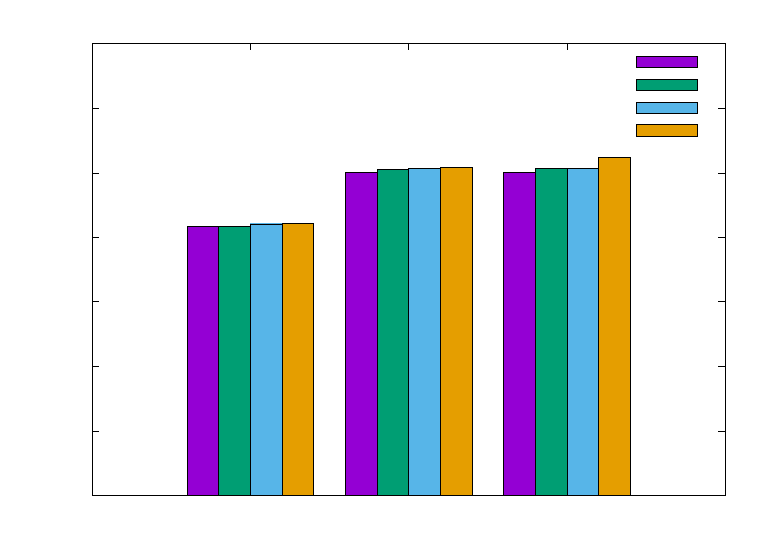
\includegraphics{chapters/chapter6/graphs/waste_environment_types}}%
    \gplfronttext
  \end{picture}%
\endgroup
}
\caption{Average and standard deviation of $\sigma $, the percentage non-prioritized items over time, for different environment types for each algorithm}
\label{fig:environmenttypesnonprioritized}
\end{figure}

In Section~\ref{experimentenvironments}, the characteristics of different environment item distributions were discussed, as well as what each environment item distribution would test in a prioritized foraging problem. 

The following hypotheses have been formulated based on those descriptions:

\begin{enumerate}
	\item The na\"ive foraging algorithm will perform better on environments with a uniform distribution compared to the clustered, vein and Gaussian environments, due to the algorithm's inability to return to areas with high item density. 
	
	\item The desert ant foraging algorithm will perform better on clustered, Gaussian and vein environments. In the desert ant foraging algorithm, robots remember location of an item source and can return quickly to areas with prioritized items.
	
	 \item The honey bee foraging algorithm will perform best on Gaussian distribution environments since robots in the honey bee foraging algorithm recruit members to forage rich prioritized item sources. 
	 
	 \item Honey bee foraging algorithm will perform worse on the uniformly distributed environments due to time wasted to recruit robots to areas which do not contain many prioritized items.
\end{enumerate}

%TODO: Insert graph and table from new results.
Table~\ref{environmenttypeprioritized} and Figure~\ref{fig:environmenttypes} show the performance of the each algorithm on each type of item distribution, with respect to $\sigma$ and $\mu$. 

% Are these valid?
The performance of each algorithm over the environment item distributions vary within a small range. Either the environment distributions are not. 


 , it is clear that suprisingly the environment types have less of an effect on performance () than expected thus one can conclude that the algorithms either do not effectively take advantage of some of the environment types or do take advantage of environment types but are hindered by other difficulties related to the environment type. 
 
 Another general and  notion across all environments is that performance of the algorithm over clustered environments seems to be similar performance of the algorithms over uniform environments. This is unexpected since, due to the fact that the clustered environment has grouped areas of prioritized items, one would expect the performance of algorithms over clustered environments to be more similar to the performance of algorithms over vein and gaussian environments since vein and gaussian environments also have grouped areas of prioritized items. The conclusion after examining a number of the environments is that the generated clustered environments do not have sparsely defined clusters and thus the clustered environments are perhaps more similar to the uniform environments. 

As expected, the na\"ive algorithm performs the best on uniform environments and the worst on gaussian and vein environments. As discussed above, the na\"ive algorithm also performs similarly on the clustered environments as it does on the uniform environments, but besides that anomaly, the first hypothesis about na\"ive environments is confirmed. 

The results presented in Table~\ref{environmenttypeprioritized} and Figure~\ref{fig:environmenttypes} surpisingly do not confirm the second hypothesis that the desert ant algorithm will perform better on the gaussian and vein environments than the uniform environments. The reason for this is actually obvious after careful thought. The uniform environment can be considered a simpler environment type than the  clustered, gaussian and vein environments since the uniform environment is less likely to result in large areas of non-prioritized items that may form larger obstacles that are difficult to navigate around. Not only that, but the uniform distribution will result in less robot-to-robot interference than gaussian and vein environments since the robots are not all trying to navigate towards the same area to locate the items and are thus likely to be evenly spread across the environment. Unlike the honey bee algorithm, which may actively be at a disadvantage in a uniform environment due to potential overhead from division of labour between foraging and resting robots and the specialization ratio division of labour, the desert ant algorithm has no such overhead. Due to the simpler nature of the uniform environment, it is thus not suprising that the desert ant algorithm performs better on the uniform environment as opposed to the more difficult vein and gaussian environments. As discussed above, the desert ant algorithm performed similarly on clustered environments as it did on uniform environments. 

The honey bee algorithm performs as expected, performing better on gaussian and environments and worse on the clustered and uniform environments. As stated above, the honey bee algorthim is actively hindered in uniform environments as it may falsely detect that the location of an environment is worth broadcasting to other robots, and thus robots are unnecessarily recruited to an area which does not have a rich concentration of prioritized items. The other problem is that there may be overhead where robots falsely switch between foraging prioritized and non-prioritized items when falsely detecting that a switch is required and thus robots end up thrashing back and forth between foraging prioritized and non-prioritized items. The honey bee algorithm is thus more suited to environments which has areas of higher concentrations of particular types of items so that division of labour does not cause unnecessary overhead and instead benefits the performance of the algorithm. 

Analysis of the average percentage of non-prioritized items foraged $\mu$ over environment types by examining Table~\ref{environmenttypenonprioritized} and Figure~\ref{fig:environmenttypesnonprioritized} confirms  that the decreased performance of the na\"ive and desert ant algorithms can likely be attributed to the difficulty of the gaussian and vein environments since the results indicate that the na\"ive and desert ant algorithms have foraged more non-prioritized items in the vein and gaussian environments than in the uniform and clustered environments. This can be attributed to the nature of the vein and gaussian environments where by the prioritized items are surrounded by a layer of non prioritized items. Thus, the swarm cannot necessarily simply navigate around the items, but will likely be forced to forage non-prioritized items in order to reach the the prioritized items. The honey bee algorithm foraged the most non-prioritized items in the vein environments which is likely due to the same reason - the robots can't navigate past the non-prioritized items and instead must forage them. 

\subsection{Item Density}
\label{results:itemdensity}

\begin{table} [h]
     \caption{Prioritized Items over Time over Item Density in Environment for each Algorithm}
     \label{itemdensityprioritized}
	\centering
	\footnotesize
	\begin{tabular} {|l|l|l|l|}
\hline
$p$ & Naive & DesertAnt & HoneyBee \\
\hline
0.05 & 0.58576 (0.397434)  & 0.709257 (0.370191)  & 0.724892 (0.331663)  \\
0.2 & 0.445301 (0.400194)  & 0.55749 (0.396821)  & 0.601527 (0.374943)  \\
0.5 & 0.34856 (0.3778)  & 0.441694 (0.395469)  & 0.494143 (0.388125)  \\
0.7 & 0.315063 (0.368166)  & 0.396919 (0.389359)  & 0.451818 (0.388338)  \\
0.9 & 0.290859 (0.360364)  & 0.365705 (0.383365)  & 0.418788 (0.38623)  \\
\hline
\end{tabular}

\end{table}

\begin{table} [h]
     \caption{Non-prioritized Items over Time over Item Density in Environment for each Algorithm}
     \label{itemdensitynonprioritized}
	\centering
	\footnotesize
	\begin{tabular} {|l|l|l|l|}
\hline
$p$ & Naive & DesertAnt & HoneyBee \\
\hline
5 & 0.620571 (0.375689)  & 0.724854 (0.353456)  & 0.712767 (0.32061)  \\
20 & 0.478558 (0.384724)  & 0.574932 (0.378252)  & 0.586206 (0.369629)  \\
50 & 0.369491 (0.367149)  & 0.451495 (0.379117)  & 0.480418 (0.379408)  \\
70 & 0.327576 (0.356324)  & 0.403477 (0.373719)  & 0.431977 (0.376965)  \\
90 & 0.29737 (0.348107)  & 0.367512 (0.368059)  & 0.39277 (0.37313)  \\
\hline
\end{tabular}

\end{table}


\begin{figure}[!htb]
\centering
\resizebox{\textwidth}{!}{% GNUPLOT: LaTeX picture with Postscript
\begingroup
  \makeatletter
  \providecommand\color[2][]{%
    \GenericError{(gnuplot) \space\space\space\@spaces}{%
      Package color not loaded in conjunction with
      terminal option `colourtext'%
    }{See the gnuplot documentation for explanation.%
    }{Either use 'blacktext' in gnuplot or load the package
      color.sty in LaTeX.}%
    \renewcommand\color[2][]{}%
  }%
  \providecommand\includegraphics[2][]{%
    \GenericError{(gnuplot) \space\space\space\@spaces}{%
      Package graphicx or graphics not loaded%
    }{See the gnuplot documentation for explanation.%
    }{The gnuplot epslatex terminal needs graphicx.sty or graphics.sty.}%
    \renewcommand\includegraphics[2][]{}%
  }%
  \providecommand\rotatebox[2]{#2}%
  \@ifundefined{ifGPcolor}{%
    \newif\ifGPcolor
    \GPcolorfalse
  }{}%
  \@ifundefined{ifGPblacktext}{%
    \newif\ifGPblacktext
    \GPblacktexttrue
  }{}%
  % define a \g@addto@macro without @ in the name:
  \let\gplgaddtomacro\g@addto@macro
  % define empty templates for all commands taking text:
  \gdef\gplbacktext{}%
  \gdef\gplfronttext{}%
  \makeatother
  \ifGPblacktext
    % no textcolor at all
    \def\colorrgb#1{}%
    \def\colorgray#1{}%
  \else
    % gray or color?
    \ifGPcolor
      \def\colorrgb#1{\color[rgb]{#1}}%
      \def\colorgray#1{\color[gray]{#1}}%
      \expandafter\def\csname LTw\endcsname{\color{white}}%
      \expandafter\def\csname LTb\endcsname{\color{black}}%
      \expandafter\def\csname LTa\endcsname{\color{black}}%
      \expandafter\def\csname LT0\endcsname{\color[rgb]{1,0,0}}%
      \expandafter\def\csname LT1\endcsname{\color[rgb]{0,1,0}}%
      \expandafter\def\csname LT2\endcsname{\color[rgb]{0,0,1}}%
      \expandafter\def\csname LT3\endcsname{\color[rgb]{1,0,1}}%
      \expandafter\def\csname LT4\endcsname{\color[rgb]{0,1,1}}%
      \expandafter\def\csname LT5\endcsname{\color[rgb]{1,1,0}}%
      \expandafter\def\csname LT6\endcsname{\color[rgb]{0,0,0}}%
      \expandafter\def\csname LT7\endcsname{\color[rgb]{1,0.3,0}}%
      \expandafter\def\csname LT8\endcsname{\color[rgb]{0.5,0.5,0.5}}%
    \else
      % gray
      \def\colorrgb#1{\color{black}}%
      \def\colorgray#1{\color[gray]{#1}}%
      \expandafter\def\csname LTw\endcsname{\color{white}}%
      \expandafter\def\csname LTb\endcsname{\color{black}}%
      \expandafter\def\csname LTa\endcsname{\color{black}}%
      \expandafter\def\csname LT0\endcsname{\color{black}}%
      \expandafter\def\csname LT1\endcsname{\color{black}}%
      \expandafter\def\csname LT2\endcsname{\color{black}}%
      \expandafter\def\csname LT3\endcsname{\color{black}}%
      \expandafter\def\csname LT4\endcsname{\color{black}}%
      \expandafter\def\csname LT5\endcsname{\color{black}}%
      \expandafter\def\csname LT6\endcsname{\color{black}}%
      \expandafter\def\csname LT7\endcsname{\color{black}}%
      \expandafter\def\csname LT8\endcsname{\color{black}}%
    \fi
  \fi
  \setlength{\unitlength}{0.0500bp}%
  \begin{picture}(7200.00,5040.00)%
    \gplgaddtomacro\gplbacktext{%
      \csname LTb\endcsname%
      \put(1078,704){\makebox(0,0)[r]{\strut{} 0.25}}%
      \put(1078,1071){\makebox(0,0)[r]{\strut{} 0.3}}%
      \put(1078,1439){\makebox(0,0)[r]{\strut{} 0.35}}%
      \put(1078,1806){\makebox(0,0)[r]{\strut{} 0.4}}%
      \put(1078,2174){\makebox(0,0)[r]{\strut{} 0.45}}%
      \put(1078,2541){\makebox(0,0)[r]{\strut{} 0.5}}%
      \put(1078,2909){\makebox(0,0)[r]{\strut{} 0.55}}%
      \put(1078,3276){\makebox(0,0)[r]{\strut{} 0.6}}%
      \put(1078,3644){\makebox(0,0)[r]{\strut{} 0.65}}%
      \put(1078,4012){\makebox(0,0)[r]{\strut{} 0.7}}%
      \put(1078,4379){\makebox(0,0)[r]{\strut{} 0.75}}%
      \put(1210,484){\makebox(0,0){\strut{} 0}}%
      \put(1831,484){\makebox(0,0){\strut{} 0.1}}%
      \put(2453,484){\makebox(0,0){\strut{} 0.2}}%
      \put(3074,484){\makebox(0,0){\strut{} 0.3}}%
      \put(3696,484){\makebox(0,0){\strut{} 0.4}}%
      \put(4317,484){\makebox(0,0){\strut{} 0.5}}%
      \put(4939,484){\makebox(0,0){\strut{} 0.6}}%
      \put(5560,484){\makebox(0,0){\strut{} 0.7}}%
      \put(6182,484){\makebox(0,0){\strut{} 0.8}}%
      \put(6803,484){\makebox(0,0){\strut{} 0.9}}%
      \put(176,2541){\rotatebox{-270}{\makebox(0,0){\strut{}Prioritized items over time ($\sigma$)}}}%
      \put(4006,154){\makebox(0,0){\strut{}Amount of Objects ($p$)}}%
      \put(4006,4709){\makebox(0,0){\strut{}Prioritized items over time for each algorithm over item density}}%
    }%
    \gplgaddtomacro\gplfronttext{%
      \csname LTb\endcsname%
      \put(5816,4206){\makebox(0,0)[r]{\strut{}Na\"ive}}%
      \csname LTb\endcsname%
      \put(5816,3986){\makebox(0,0)[r]{\strut{}Desert Ant}}%
      \csname LTb\endcsname%
      \put(5816,3766){\makebox(0,0)[r]{\strut{}Honey Bee}}%
    }%
    \gplbacktext
    \put(0,0){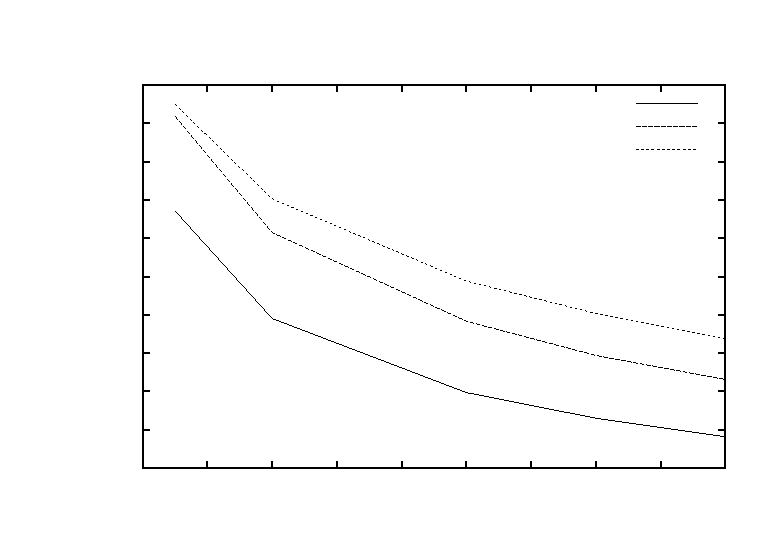
\includegraphics{chapters/chapter6/graphs/gold_objects}}%
    \gplfronttext
  \end{picture}%
\endgroup
}
\caption{Prioritized Items over Time over Item Density in Environment  for each Algorithm}
\label{objectgoldplot}
\end{figure}


\begin{figure}[!htb]
\centering
\resizebox{\textwidth}{!}{% GNUPLOT: LaTeX picture with Postscript
\begingroup
  \makeatletter
  \providecommand\color[2][]{%
    \GenericError{(gnuplot) \space\space\space\@spaces}{%
      Package color not loaded in conjunction with
      terminal option `colourtext'%
    }{See the gnuplot documentation for explanation.%
    }{Either use 'blacktext' in gnuplot or load the package
      color.sty in LaTeX.}%
    \renewcommand\color[2][]{}%
  }%
  \providecommand\includegraphics[2][]{%
    \GenericError{(gnuplot) \space\space\space\@spaces}{%
      Package graphicx or graphics not loaded%
    }{See the gnuplot documentation for explanation.%
    }{The gnuplot epslatex terminal needs graphicx.sty or graphics.sty.}%
    \renewcommand\includegraphics[2][]{}%
  }%
  \providecommand\rotatebox[2]{#2}%
  \@ifundefined{ifGPcolor}{%
    \newif\ifGPcolor
    \GPcolorfalse
  }{}%
  \@ifundefined{ifGPblacktext}{%
    \newif\ifGPblacktext
    \GPblacktexttrue
  }{}%
  % define a \g@addto@macro without @ in the name:
  \let\gplgaddtomacro\g@addto@macro
  % define empty templates for all commands taking text:
  \gdef\gplbacktext{}%
  \gdef\gplfronttext{}%
  \makeatother
  \ifGPblacktext
    % no textcolor at all
    \def\colorrgb#1{}%
    \def\colorgray#1{}%
  \else
    % gray or color?
    \ifGPcolor
      \def\colorrgb#1{\color[rgb]{#1}}%
      \def\colorgray#1{\color[gray]{#1}}%
      \expandafter\def\csname LTw\endcsname{\color{white}}%
      \expandafter\def\csname LTb\endcsname{\color{black}}%
      \expandafter\def\csname LTa\endcsname{\color{black}}%
      \expandafter\def\csname LT0\endcsname{\color[rgb]{1,0,0}}%
      \expandafter\def\csname LT1\endcsname{\color[rgb]{0,1,0}}%
      \expandafter\def\csname LT2\endcsname{\color[rgb]{0,0,1}}%
      \expandafter\def\csname LT3\endcsname{\color[rgb]{1,0,1}}%
      \expandafter\def\csname LT4\endcsname{\color[rgb]{0,1,1}}%
      \expandafter\def\csname LT5\endcsname{\color[rgb]{1,1,0}}%
      \expandafter\def\csname LT6\endcsname{\color[rgb]{0,0,0}}%
      \expandafter\def\csname LT7\endcsname{\color[rgb]{1,0.3,0}}%
      \expandafter\def\csname LT8\endcsname{\color[rgb]{0.5,0.5,0.5}}%
    \else
      % gray
      \def\colorrgb#1{\color{black}}%
      \def\colorgray#1{\color[gray]{#1}}%
      \expandafter\def\csname LTw\endcsname{\color{white}}%
      \expandafter\def\csname LTb\endcsname{\color{black}}%
      \expandafter\def\csname LTa\endcsname{\color{black}}%
      \expandafter\def\csname LT0\endcsname{\color{black}}%
      \expandafter\def\csname LT1\endcsname{\color{black}}%
      \expandafter\def\csname LT2\endcsname{\color{black}}%
      \expandafter\def\csname LT3\endcsname{\color{black}}%
      \expandafter\def\csname LT4\endcsname{\color{black}}%
      \expandafter\def\csname LT5\endcsname{\color{black}}%
      \expandafter\def\csname LT6\endcsname{\color{black}}%
      \expandafter\def\csname LT7\endcsname{\color{black}}%
      \expandafter\def\csname LT8\endcsname{\color{black}}%
    \fi
  \fi
  \setlength{\unitlength}{0.0500bp}%
  \begin{picture}(7200.00,5040.00)%
    \gplgaddtomacro\gplbacktext{%
      \csname LTb\endcsname%
      \put(946,704){\makebox(0,0)[r]{\strut{} 0.3}}%
      \put(946,1229){\makebox(0,0)[r]{\strut{} 0.4}}%
      \put(946,1754){\makebox(0,0)[r]{\strut{} 0.5}}%
      \put(946,2279){\makebox(0,0)[r]{\strut{} 0.6}}%
      \put(946,2804){\makebox(0,0)[r]{\strut{} 0.7}}%
      \put(946,3329){\makebox(0,0)[r]{\strut{} 0.8}}%
      \put(946,3854){\makebox(0,0)[r]{\strut{} 0.9}}%
      \put(946,4379){\makebox(0,0)[r]{\strut{} 1}}%
      \put(1078,484){\makebox(0,0){\strut{} 0}}%
      \put(2223,484){\makebox(0,0){\strut{} 0.2}}%
      \put(3368,484){\makebox(0,0){\strut{} 0.4}}%
      \put(4513,484){\makebox(0,0){\strut{} 0.6}}%
      \put(5658,484){\makebox(0,0){\strut{} 0.8}}%
      \put(6803,484){\makebox(0,0){\strut{} 1}}%
      \put(176,2541){\rotatebox{-270}{\makebox(0,0){\strut{}Non-prioritized items over time ($\sigma$)}}}%
      \put(3940,154){\makebox(0,0){\strut{}Amount of Objects ($p$)}}%
      \put(3940,4709){\makebox(0,0){\strut{}Non-prioritized items over time for each algorithm over object percentages}}%
    }%
    \gplgaddtomacro\gplfronttext{%
      \csname LTb\endcsname%
      \put(5816,4206){\makebox(0,0)[r]{\strut{}Na\"ive}}%
      \csname LTb\endcsname%
      \put(5816,3986){\makebox(0,0)[r]{\strut{}Desert Ant}}%
      \csname LTb\endcsname%
      \put(5816,3766){\makebox(0,0)[r]{\strut{}Honey Bee}}%
    }%
    \gplbacktext
    \put(0,0){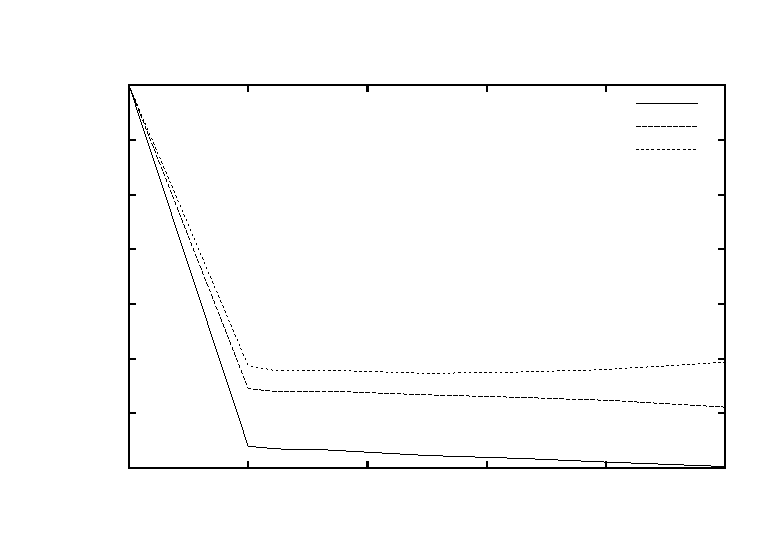
\includegraphics{chapters/chapter6/graphs/waste_objects}}%
    \gplfronttext
  \end{picture}%
\endgroup
}
\caption{Non-prioritized Items over Time over Item Density in Environment for each Algorithm}
\label{objectwasteplot}
\end{figure}

Item density is examined in order to determine if algorithm performance is affected y an increase in environment complexity. As the density of items increases, the more difficult navigation becomes around non-prioritized items that form obstalces when there isn't a suitable specialization ratio of robots. Conversely however, the more dense the enviroment's are then the richer and denser the deposits of prioritized items may becomes in certain environments, thus the division of labour of the honey bee algorithm may become more effective at higher densities. As indicated in \ref{objectgoldplot}, all algorithms are shown to degrade quite heavily as the items density increases. This is to be expected as it will take longer for robots to forage all items in the denser environment. Thus the degradation of performance can likely be attributed to the limit on simulation time which should have been extended in order to cater for the large environments. Unfortunately, to adequately compare and analyse the performance as item density increases, one would have to allow more time over all to simulations.

\section{Robustness}
\label{results:robustness}

Robustness can be defined as an algorithms ability to degrade gracefully or recover from damage or malfunction to of a portion of the swarm. A robust algorithms performance should thus be independant of any specific initial swarm configuration such as the specialization ratio. The more homogenous the swarm, in general, the more robust the swarm will be to failure of a portion of the swarm since the swarm will not have any dependancies on a specific individual or group of individuals within the swarm. The less homogenous the swarm is, the most likely the swarm will suffer when individuals with specific capabilities malfunction or are damaged.

\subsection{Swarm Specialization}
\label{results:specialization}

The reason the initial swarm specialization ratio has been included under robustness is that the more dependant the algorithm is to swarm specialization ratio, the more sensitive  the algorithm is to robots becoming damaged. When referring to specialization in this chapter, it is referring specifically to the initial swarm specialization ratio $\tau$ of the swarm of robots. 

\begin{table} [h]
     \caption{Prioritized Items over Time over Swarm Specialization Ratio for each Algorithm}
     \label{specializationprioritized}
	\centering
	\footnotesize
	\begin{tabular} {|l|l|l|l|}
\hline
$\tau$ & Naive & DesertAnt & HoneyBee \\
\hline
0 & 0.111111 (0.314271)  & 0.111111 (0.314271)  & 0.537741 (0.390935)  \\
0.2 & 0.36135 (0.377053)  & 0.47583 (0.389053)  & 0.538168 (0.390927)  \\
0.25 & 0.384587 (0.381465)  & 0.506607 (0.391131)  & 0.538193 (0.390901)  \\
0.333333 & 0.413082 (0.386904)  & 0.53241 (0.389767)  & 0.538255 (0.390877)  \\
0.5 & 0.448139 (0.3905)  & 0.564046 (0.387498)  & 0.538318 (0.390842)  \\
0.666667 & 0.467119 (0.392242)  & 0.577736 (0.386812)  & 0.538339 (0.3908)  \\
0.75 & 0.470999 (0.392544)  & 0.578073 (0.387456)  & 0.538502 (0.390756)  \\
0.8 & 0.471725 (0.392973)  & 0.570267 (0.388001)  & 0.537496 (0.39078)  \\
1 & 0.445866 (0.395946)  & 0.531837 (0.401191)  & 0.539093 (0.390633)  \\
\hline
\end{tabular}

\end{table}

\begin{table} [h]
     \caption{Non-prioritized Items over Time over Swarm Specialization Ratio for each Algorithm}
     \label{specializationnonprioritized}
	\centering
	\footnotesize
	\begin{tabular} {|l|l|l|l|}
\hline
$\tau$ & Naive & DesertAnt & HoneyBee \\
\hline
0 & 0.476407 (0.375128)  & 0.554143 (0.375166)  & 0.521633 (0.382233)  \\
0.2 & 0.490862 (0.372655)  & 0.588561 (0.365842)  & 0.521377 (0.382389)  \\
0.25 & 0.490406 (0.373393)  & 0.590359 (0.366179)  & 0.521327 (0.382381)  \\
0.333333 & 0.486581 (0.374537)  & 0.58901 (0.367036)  & 0.521319 (0.382432)  \\
0.5 & 0.470841 (0.375931)  & 0.575395 (0.370063)  & 0.521078 (0.382581)  \\
0.666667 & 0.438305 (0.375474)  & 0.538074 (0.375264)  & 0.520765 (0.382733)  \\
0.75 & 0.413096 (0.373736)  & 0.510426 (0.376969)  & 0.52061 (0.382775)  \\
0.8 & 0.390809 (0.372202)  & 0.483009 (0.377386)  & 0.517882 (0.382866)  \\
1 & 0.111111 (0.314271)  & 0.111111 (0.314271)  & 0.521457 (0.382585)  \\
\hline
\end{tabular}

\end{table}

\begin{figure}[!htb]
\centering
\resizebox{\textwidth}{!}{% GNUPLOT: LaTeX picture with Postscript
\begingroup
  \makeatletter
  \providecommand\color[2][]{%
    \GenericError{(gnuplot) \space\space\space\@spaces}{%
      Package color not loaded in conjunction with
      terminal option `colourtext'%
    }{See the gnuplot documentation for explanation.%
    }{Either use 'blacktext' in gnuplot or load the package
      color.sty in LaTeX.}%
    \renewcommand\color[2][]{}%
  }%
  \providecommand\includegraphics[2][]{%
    \GenericError{(gnuplot) \space\space\space\@spaces}{%
      Package graphicx or graphics not loaded%
    }{See the gnuplot documentation for explanation.%
    }{The gnuplot epslatex terminal needs graphicx.sty or graphics.sty.}%
    \renewcommand\includegraphics[2][]{}%
  }%
  \providecommand\rotatebox[2]{#2}%
  \@ifundefined{ifGPcolor}{%
    \newif\ifGPcolor
    \GPcolorfalse
  }{}%
  \@ifundefined{ifGPblacktext}{%
    \newif\ifGPblacktext
    \GPblacktexttrue
  }{}%
  % define a \g@addto@macro without @ in the name:
  \let\gplgaddtomacro\g@addto@macro
  % define empty templates for all commands taking text:
  \gdef\gplbacktext{}%
  \gdef\gplfronttext{}%
  \makeatother
  \ifGPblacktext
    % no textcolor at all
    \def\colorrgb#1{}%
    \def\colorgray#1{}%
  \else
    % gray or color?
    \ifGPcolor
      \def\colorrgb#1{\color[rgb]{#1}}%
      \def\colorgray#1{\color[gray]{#1}}%
      \expandafter\def\csname LTw\endcsname{\color{white}}%
      \expandafter\def\csname LTb\endcsname{\color{black}}%
      \expandafter\def\csname LTa\endcsname{\color{black}}%
      \expandafter\def\csname LT0\endcsname{\color[rgb]{1,0,0}}%
      \expandafter\def\csname LT1\endcsname{\color[rgb]{0,1,0}}%
      \expandafter\def\csname LT2\endcsname{\color[rgb]{0,0,1}}%
      \expandafter\def\csname LT3\endcsname{\color[rgb]{1,0,1}}%
      \expandafter\def\csname LT4\endcsname{\color[rgb]{0,1,1}}%
      \expandafter\def\csname LT5\endcsname{\color[rgb]{1,1,0}}%
      \expandafter\def\csname LT6\endcsname{\color[rgb]{0,0,0}}%
      \expandafter\def\csname LT7\endcsname{\color[rgb]{1,0.3,0}}%
      \expandafter\def\csname LT8\endcsname{\color[rgb]{0.5,0.5,0.5}}%
    \else
      % gray
      \def\colorrgb#1{\color{black}}%
      \def\colorgray#1{\color[gray]{#1}}%
      \expandafter\def\csname LTw\endcsname{\color{white}}%
      \expandafter\def\csname LTb\endcsname{\color{black}}%
      \expandafter\def\csname LTa\endcsname{\color{black}}%
      \expandafter\def\csname LT0\endcsname{\color{black}}%
      \expandafter\def\csname LT1\endcsname{\color{black}}%
      \expandafter\def\csname LT2\endcsname{\color{black}}%
      \expandafter\def\csname LT3\endcsname{\color{black}}%
      \expandafter\def\csname LT4\endcsname{\color{black}}%
      \expandafter\def\csname LT5\endcsname{\color{black}}%
      \expandafter\def\csname LT6\endcsname{\color{black}}%
      \expandafter\def\csname LT7\endcsname{\color{black}}%
      \expandafter\def\csname LT8\endcsname{\color{black}}%
    \fi
  \fi
  \setlength{\unitlength}{0.0500bp}%
  \begin{picture}(7200.00,5040.00)%
    \gplgaddtomacro\gplbacktext{%
      \csname LTb\endcsname%
      \put(1078,704){\makebox(0,0)[r]{\strut{} 0.1}}%
      \put(1078,1072){\makebox(0,0)[r]{\strut{} 0.15}}%
      \put(1078,1439){\makebox(0,0)[r]{\strut{} 0.2}}%
      \put(1078,1806){\makebox(0,0)[r]{\strut{} 0.25}}%
      \put(1078,2174){\makebox(0,0)[r]{\strut{} 0.3}}%
      \put(1078,2541){\makebox(0,0)[r]{\strut{} 0.35}}%
      \put(1078,2909){\makebox(0,0)[r]{\strut{} 0.4}}%
      \put(1078,3276){\makebox(0,0)[r]{\strut{} 0.45}}%
      \put(1078,3644){\makebox(0,0)[r]{\strut{} 0.5}}%
      \put(1078,4011){\makebox(0,0)[r]{\strut{} 0.55}}%
      \put(1078,4379){\makebox(0,0)[r]{\strut{} 0.6}}%
      \put(1210,484){\makebox(0,0){\strut{} 0}}%
      \put(2329,484){\makebox(0,0){\strut{} 0.2}}%
      \put(3447,484){\makebox(0,0){\strut{} 0.4}}%
      \put(4566,484){\makebox(0,0){\strut{} 0.6}}%
      \put(5684,484){\makebox(0,0){\strut{} 0.8}}%
      \put(6803,484){\makebox(0,0){\strut{} 1}}%
      \put(176,2541){\rotatebox{-270}{\makebox(0,0){\strut{}Prioritized items over time ($\sigma$)}}}%
      \put(4006,154){\makebox(0,0){\strut{}Robot Type Ratio ($r$)}}%
      \put(4006,4709){\makebox(0,0){\strut{}Prioritized items over time for each algorithm for robot type ratios}}%
    }%
    \gplgaddtomacro\gplfronttext{%
      \csname LTb\endcsname%
      \put(5816,4206){\makebox(0,0)[r]{\strut{}Na\"ive}}%
      \csname LTb\endcsname%
      \put(5816,3986){\makebox(0,0)[r]{\strut{}Desert Ant}}%
      \csname LTb\endcsname%
      \put(5816,3766){\makebox(0,0)[r]{\strut{}Honey Bee}}%
    }%
    \gplbacktext
    \put(0,0){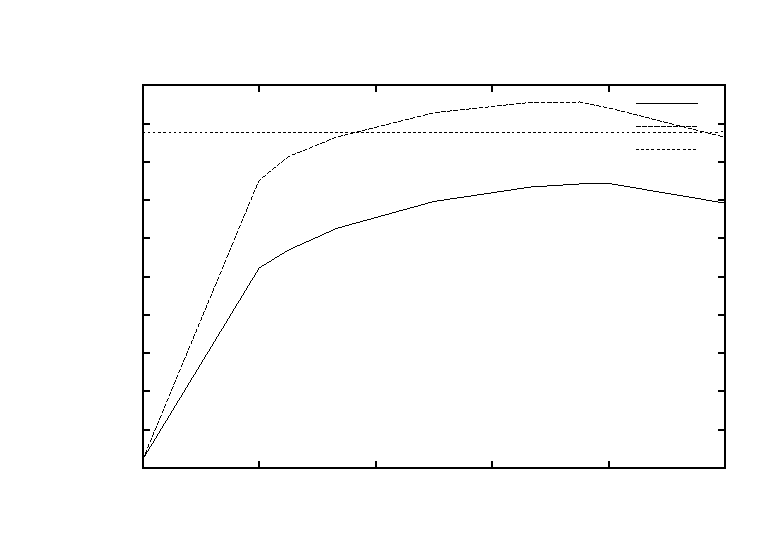
\includegraphics{chapters/chapter6/graphs/gold_division}}%
    \gplfronttext
  \end{picture}%
\endgroup
}
\caption{Prioritized items over time over specialization ratio $\tau$ for each algorithm }
\label{divisiongoldplot}
\end{figure}

\begin{figure}[!htb]
\centering
\resizebox{\textwidth}{!}{% GNUPLOT: LaTeX picture with Postscript
\begingroup
  \makeatletter
  \providecommand\color[2][]{%
    \GenericError{(gnuplot) \space\space\space\@spaces}{%
      Package color not loaded in conjunction with
      terminal option `colourtext'%
    }{See the gnuplot documentation for explanation.%
    }{Either use 'blacktext' in gnuplot or load the package
      color.sty in LaTeX.}%
    \renewcommand\color[2][]{}%
  }%
  \providecommand\includegraphics[2][]{%
    \GenericError{(gnuplot) \space\space\space\@spaces}{%
      Package graphicx or graphics not loaded%
    }{See the gnuplot documentation for explanation.%
    }{The gnuplot epslatex terminal needs graphicx.sty or graphics.sty.}%
    \renewcommand\includegraphics[2][]{}%
  }%
  \providecommand\rotatebox[2]{#2}%
  \@ifundefined{ifGPcolor}{%
    \newif\ifGPcolor
    \GPcolorfalse
  }{}%
  \@ifundefined{ifGPblacktext}{%
    \newif\ifGPblacktext
    \GPblacktexttrue
  }{}%
  % define a \g@addto@macro without @ in the name:
  \let\gplgaddtomacro\g@addto@macro
  % define empty templates for all commands taking text:
  \gdef\gplbacktext{}%
  \gdef\gplfronttext{}%
  \makeatother
  \ifGPblacktext
    % no textcolor at all
    \def\colorrgb#1{}%
    \def\colorgray#1{}%
  \else
    % gray or color?
    \ifGPcolor
      \def\colorrgb#1{\color[rgb]{#1}}%
      \def\colorgray#1{\color[gray]{#1}}%
      \expandafter\def\csname LTw\endcsname{\color{white}}%
      \expandafter\def\csname LTb\endcsname{\color{black}}%
      \expandafter\def\csname LTa\endcsname{\color{black}}%
      \expandafter\def\csname LT0\endcsname{\color[rgb]{1,0,0}}%
      \expandafter\def\csname LT1\endcsname{\color[rgb]{0,1,0}}%
      \expandafter\def\csname LT2\endcsname{\color[rgb]{0,0,1}}%
      \expandafter\def\csname LT3\endcsname{\color[rgb]{1,0,1}}%
      \expandafter\def\csname LT4\endcsname{\color[rgb]{0,1,1}}%
      \expandafter\def\csname LT5\endcsname{\color[rgb]{1,1,0}}%
      \expandafter\def\csname LT6\endcsname{\color[rgb]{0,0,0}}%
      \expandafter\def\csname LT7\endcsname{\color[rgb]{1,0.3,0}}%
      \expandafter\def\csname LT8\endcsname{\color[rgb]{0.5,0.5,0.5}}%
    \else
      % gray
      \def\colorrgb#1{\color{black}}%
      \def\colorgray#1{\color[gray]{#1}}%
      \expandafter\def\csname LTw\endcsname{\color{white}}%
      \expandafter\def\csname LTb\endcsname{\color{black}}%
      \expandafter\def\csname LTa\endcsname{\color{black}}%
      \expandafter\def\csname LT0\endcsname{\color{black}}%
      \expandafter\def\csname LT1\endcsname{\color{black}}%
      \expandafter\def\csname LT2\endcsname{\color{black}}%
      \expandafter\def\csname LT3\endcsname{\color{black}}%
      \expandafter\def\csname LT4\endcsname{\color{black}}%
      \expandafter\def\csname LT5\endcsname{\color{black}}%
      \expandafter\def\csname LT6\endcsname{\color{black}}%
      \expandafter\def\csname LT7\endcsname{\color{black}}%
      \expandafter\def\csname LT8\endcsname{\color{black}}%
    \fi
  \fi
  \setlength{\unitlength}{0.0500bp}%
  \begin{picture}(7200.00,5040.00)%
    \gplgaddtomacro\gplbacktext{%
      \csname LTb\endcsname%
      \put(1078,704){\makebox(0,0)[r]{\strut{} 0.1}}%
      \put(1078,1072){\makebox(0,0)[r]{\strut{} 0.15}}%
      \put(1078,1439){\makebox(0,0)[r]{\strut{} 0.2}}%
      \put(1078,1806){\makebox(0,0)[r]{\strut{} 0.25}}%
      \put(1078,2174){\makebox(0,0)[r]{\strut{} 0.3}}%
      \put(1078,2541){\makebox(0,0)[r]{\strut{} 0.35}}%
      \put(1078,2909){\makebox(0,0)[r]{\strut{} 0.4}}%
      \put(1078,3276){\makebox(0,0)[r]{\strut{} 0.45}}%
      \put(1078,3644){\makebox(0,0)[r]{\strut{} 0.5}}%
      \put(1078,4011){\makebox(0,0)[r]{\strut{} 0.55}}%
      \put(1078,4379){\makebox(0,0)[r]{\strut{} 0.6}}%
      \put(1210,484){\makebox(0,0){\strut{} 0}}%
      \put(2329,484){\makebox(0,0){\strut{} 0.2}}%
      \put(3447,484){\makebox(0,0){\strut{} 0.4}}%
      \put(4566,484){\makebox(0,0){\strut{} 0.6}}%
      \put(5684,484){\makebox(0,0){\strut{} 0.8}}%
      \put(6803,484){\makebox(0,0){\strut{} 1}}%
      \put(176,2541){\rotatebox{-270}{\makebox(0,0){\strut{}Non-prioritized items over time ($\tau$)}}}%
      \put(4006,154){\makebox(0,0){\strut{}Robot Specialization Ratio($\tau$)}}%
      \put(4006,4709){\makebox(0,0){\strut{}Non-prioritized items over time for each algorithm for robot specialization ratios}}%
    }%
    \gplgaddtomacro\gplfronttext{%
      \csname LTb\endcsname%
      \put(5816,4206){\makebox(0,0)[r]{\strut{}Na\"ive}}%
      \csname LTb\endcsname%
      \put(5816,3986){\makebox(0,0)[r]{\strut{}Desert Ant}}%
      \csname LTb\endcsname%
      \put(5816,3766){\makebox(0,0)[r]{\strut{}Honey Bee}}%
    }%
    \gplbacktext
    \put(0,0){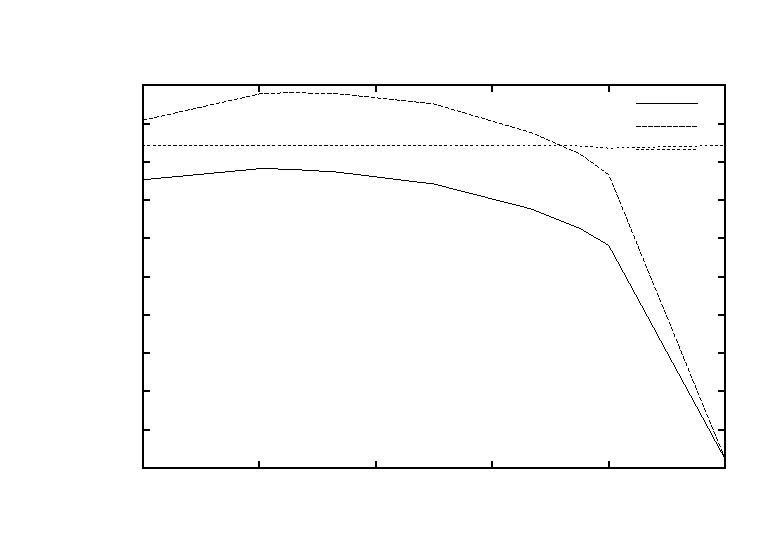
\includegraphics{chapters/chapter6/graphs/waste_division}}%
    \gplfronttext
  \end{picture}%
\endgroup
}
\caption{Non-prioritized items over time over specialization ratio $\tau$ for each algorithm}
\label{divisionwasteplot}
\end{figure}

An examination of Figure~\ref{divisiongoldplot} and Figure~\ref{divisionwasteplot} reveals some surprising observations.
As was discussed in Section~\ref{results:flexibility}, the overall trend is that as the ratio of robots foraging the prioritized type increases, the performance of the na\"ive algorithm increases. An interesting observation is that a swarm specialization ratio $r=0.8$ results in the best performance for the na\"ive foraging aglorithms, while $r=1$, where all robots are foraging prioritized items, has slightly less effective performance. This can be attributed to the fact that foraging a portion of non-prioritized items benefits the algorithm.

%Discuss Desert Ant
The desert ant algorithm shows similar trends to the na\"ive algorithm with performance peaking around $r=0.8$ while the honey bee algorithm is consistent over specialization, indicating that the honey bee algorithm does indeed perform division of labour to some level of adequacy. The desert ant does however outperform the honey bee algorithm on most of the configurations. There is space for the honey bee algorithm to be optimized so to more adequately compare the algorithms, one would have to optimize the parameters. 
The performance of desert ant algorithm is interesting since there exists a configuration for $r$, $r=0.8$ that results in the best performance, independent of all environment types. That performance is better than the honey bee performance which means that a swarm of robots running the desert ant algorithm with the correct specialization ratio of robots will perform better than a honey bee algorithm at any swarm specialization ratio. 

The desert ant algorithm, however, is less robust since if an event causes a change in robot specialization ratio (for example robots becoming damaged in a rock fall), the performance of the desert ant algorithm will be affected by the change in ratio, where as the honey bee algorithm performance would remain constant due to the division of labour and it's attempts to optimize (albeit sub-optimally) the specialization ratio of robots. 

The result does make one wonder why none of the other graphs reflect the fact that the honey bee algorithm is outperformed by the desert ant algorithm. The other results and graphs in this study are most likely skewed by the experiments when $r=0$ where no desert ant robots can forage prioritized items and thus when examining results aggregated over a different parameter, the results are skewed. One should note that since the study is not focused on a comparison of performance of the various foraging algorithms, but rather an exploration in parameter sensitivity, the relative performance of the algorithms to each other is not important, however it is still an interesting result considering that since the honey bee agents can share information as well as divide their labour appropriately. 
 
Some possible reasons why the desert ant algorithm may outperform the honey bee algorithm are that:
\begin{enumerate}
	\item The honey bee division of labour does not perfectly divide labour between the item types.
	\item Honey bee algorithm has a limiting factor such as one of the unoptimized parameters $f_{max}$ and $t_{max}$. 
	\item The process of the division of labour is slowing down the algorithm to some degree.
\end{enumerate}

In terms of robustness, despite the desert ant outperforming the honey bee algorithm on certain configurations, the fact that performance of the desert ant algorithm is dependant on the initial specialization ratio of the swarm indicates that the desert ant algorithm is less robust since if large portion of robots are damaged, and the specialization ratio is thus changed, the algorithms performance may decrease significantly. The honey bee algorithm can adjust the specialization ratio of the swarm to a near optimal configuration and thus if damange to the robots causes a change in specialization ratio, the algorithm should have the ability to adapt the specialization ratio in order to maintain a gracefully degraded performance. The performance of na\"ive algorithm, similarly to the performance of desert ant algorithm is also dependant on the initial specializtion ratio as can be seen in Figure~\ref{divisiongoldplot} and Figure~\ref{divisionwasteplot}. 

\section{Scalability}
\label{results:scability}
Scalability is a key feature of swarm robotics. In order to examine the scalability of the proposed foraging algorithms, the performance of algorithms is compared over differing swarm densities. 

\subsection{Swarm Density}
\label{results:numberenvironments}

\begin{table} [h]
     \caption{Prioritized Items over Time over Swarm Density for each Algorithm}
     \label{specializationprioritized}
	\centering
	\footnotesize
	\begin{tabular} {|l|l|l|l|}
\hline
robots & Naive & DesertAnt & HoneyBee \\
\hline
10 & 0.265658 (0.354152)  & 0.353458 (0.379052)  & 0.361346 (0.366448)  \\
30 & 0.368033 (0.382883)  & 0.465996 (0.403473)  & 0.506498 (0.388872)  \\
50 & 0.418804 (0.396546)  & 0.51716 (0.405535)  & 0.569589 (0.384909)  \\
70 & 0.450645 (0.402438)  & 0.550065 (0.404444)  & 0.607577 (0.377375)  \\
100 & 0.482404 (0.40568)  & 0.584385 (0.401958)  & 0.646158 (0.371379)  \\
\hline
\end{tabular}

\end{table}
\begin{figure}[!htb]
\centering
\resizebox{\textwidth}{!}{% GNUPLOT: LaTeX picture with Postscript
\begingroup
  \makeatletter
  \providecommand\color[2][]{%
    \GenericError{(gnuplot) \space\space\space\@spaces}{%
      Package color not loaded in conjunction with
      terminal option `colourtext'%
    }{See the gnuplot documentation for explanation.%
    }{Either use 'blacktext' in gnuplot or load the package
      color.sty in LaTeX.}%
    \renewcommand\color[2][]{}%
  }%
  \providecommand\includegraphics[2][]{%
    \GenericError{(gnuplot) \space\space\space\@spaces}{%
      Package graphicx or graphics not loaded%
    }{See the gnuplot documentation for explanation.%
    }{The gnuplot epslatex terminal needs graphicx.sty or graphics.sty.}%
    \renewcommand\includegraphics[2][]{}%
  }%
  \providecommand\rotatebox[2]{#2}%
  \@ifundefined{ifGPcolor}{%
    \newif\ifGPcolor
    \GPcolorfalse
  }{}%
  \@ifundefined{ifGPblacktext}{%
    \newif\ifGPblacktext
    \GPblacktexttrue
  }{}%
  % define a \g@addto@macro without @ in the name:
  \let\gplgaddtomacro\g@addto@macro
  % define empty templates for all commands taking text:
  \gdef\gplbacktext{}%
  \gdef\gplfronttext{}%
  \makeatother
  \ifGPblacktext
    % no textcolor at all
    \def\colorrgb#1{}%
    \def\colorgray#1{}%
  \else
    % gray or color?
    \ifGPcolor
      \def\colorrgb#1{\color[rgb]{#1}}%
      \def\colorgray#1{\color[gray]{#1}}%
      \expandafter\def\csname LTw\endcsname{\color{white}}%
      \expandafter\def\csname LTb\endcsname{\color{black}}%
      \expandafter\def\csname LTa\endcsname{\color{black}}%
      \expandafter\def\csname LT0\endcsname{\color[rgb]{1,0,0}}%
      \expandafter\def\csname LT1\endcsname{\color[rgb]{0,1,0}}%
      \expandafter\def\csname LT2\endcsname{\color[rgb]{0,0,1}}%
      \expandafter\def\csname LT3\endcsname{\color[rgb]{1,0,1}}%
      \expandafter\def\csname LT4\endcsname{\color[rgb]{0,1,1}}%
      \expandafter\def\csname LT5\endcsname{\color[rgb]{1,1,0}}%
      \expandafter\def\csname LT6\endcsname{\color[rgb]{0,0,0}}%
      \expandafter\def\csname LT7\endcsname{\color[rgb]{1,0.3,0}}%
      \expandafter\def\csname LT8\endcsname{\color[rgb]{0.5,0.5,0.5}}%
    \else
      % gray
      \def\colorrgb#1{\color{black}}%
      \def\colorgray#1{\color[gray]{#1}}%
      \expandafter\def\csname LTw\endcsname{\color{white}}%
      \expandafter\def\csname LTb\endcsname{\color{black}}%
      \expandafter\def\csname LTa\endcsname{\color{black}}%
      \expandafter\def\csname LT0\endcsname{\color{black}}%
      \expandafter\def\csname LT1\endcsname{\color{black}}%
      \expandafter\def\csname LT2\endcsname{\color{black}}%
      \expandafter\def\csname LT3\endcsname{\color{black}}%
      \expandafter\def\csname LT4\endcsname{\color{black}}%
      \expandafter\def\csname LT5\endcsname{\color{black}}%
      \expandafter\def\csname LT6\endcsname{\color{black}}%
      \expandafter\def\csname LT7\endcsname{\color{black}}%
      \expandafter\def\csname LT8\endcsname{\color{black}}%
    \fi
  \fi
  \setlength{\unitlength}{0.0500bp}%
  \begin{picture}(7200.00,5040.00)%
    \gplgaddtomacro\gplbacktext{%
      \csname LTb\endcsname%
      \put(1078,704){\makebox(0,0)[r]{\strut{} 0.25}}%
      \put(1078,1163){\makebox(0,0)[r]{\strut{} 0.3}}%
      \put(1078,1623){\makebox(0,0)[r]{\strut{} 0.35}}%
      \put(1078,2082){\makebox(0,0)[r]{\strut{} 0.4}}%
      \put(1078,2541){\makebox(0,0)[r]{\strut{} 0.45}}%
      \put(1078,3001){\makebox(0,0)[r]{\strut{} 0.5}}%
      \put(1078,3460){\makebox(0,0)[r]{\strut{} 0.55}}%
      \put(1078,3920){\makebox(0,0)[r]{\strut{} 0.6}}%
      \put(1078,4379){\makebox(0,0)[r]{\strut{} 0.65}}%
      \put(1210,484){\makebox(0,0){\strut{} 0.1}}%
      \put(1831,484){\makebox(0,0){\strut{} 0.2}}%
      \put(2453,484){\makebox(0,0){\strut{} 0.3}}%
      \put(3074,484){\makebox(0,0){\strut{} 0.4}}%
      \put(3696,484){\makebox(0,0){\strut{} 0.5}}%
      \put(4317,484){\makebox(0,0){\strut{} 0.6}}%
      \put(4939,484){\makebox(0,0){\strut{} 0.7}}%
      \put(5560,484){\makebox(0,0){\strut{} 0.8}}%
      \put(6182,484){\makebox(0,0){\strut{} 0.9}}%
      \put(6803,484){\makebox(0,0){\strut{} 1.0}}%
      \put(176,2541){\rotatebox{-270}{\makebox(0,0){\strut{}Prioritized items over time ($\sigma$)}}}%
      \put(4006,154){\makebox(0,0){\strut{}Swarm Density($c$)}}%
      \put(4006,4709){\makebox(0,0){\strut{}Prioritized items over time for each algorithm over swarm density}}%
    }%
    \gplgaddtomacro\gplfronttext{%
      \csname LTb\endcsname%
      \put(5816,4206){\makebox(0,0)[r]{\strut{}Na\"ive}}%
      \csname LTb\endcsname%
      \put(5816,3986){\makebox(0,0)[r]{\strut{}Desert Ant}}%
      \csname LTb\endcsname%
      \put(5816,3766){\makebox(0,0)[r]{\strut{}Honey Bee}}%
    }%
    \gplbacktext
    \put(0,0){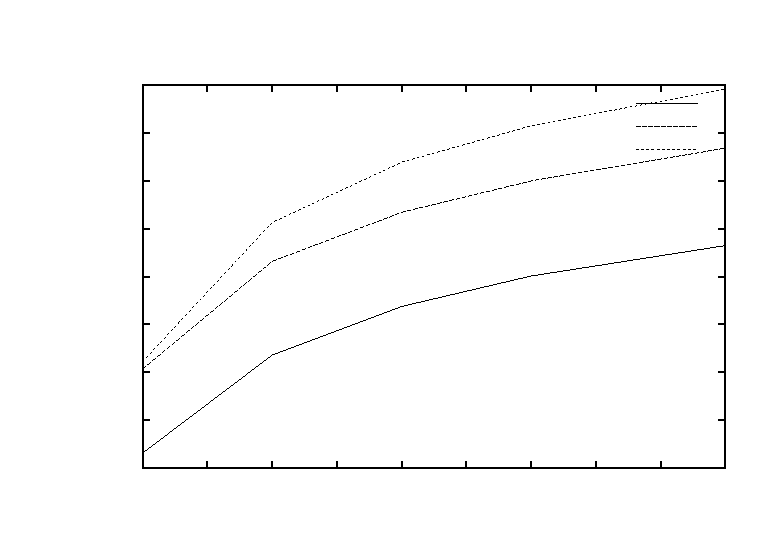
\includegraphics{chapters/chapter6/graphs/gold_robots}}%
    \gplfronttext
  \end{picture}%
\endgroup
}
\caption{Prioritized items over time over Swarm Density($c$)}
\label{robotsgoldplot}
\end{figure}

\begin{table} [h]
     \caption{Non-prioritized Items over Time over Swarm Density for each Algorithm}
     \label{specializationnonprioritized}
	\centering
	\footnotesize
	\begin{tabular} {|l|l|l|l|}
\hline
robots & Naive & DesertAnt & HoneyBee \\
\hline
10 & 0.291567 (0.352044)  & 0.356625 (0.364772)  & 0.345211 (0.356824)  \\
30 & 0.389567 (0.372173)  & 0.476672 (0.388565)  & 0.491426 (0.377163)  \\
50 & 0.439592 (0.383808)  & 0.529349 (0.390192)  & 0.553847 (0.377417)  \\
70 & 0.471239 (0.389444)  & 0.562602 (0.388846)  & 0.588479 (0.370034)  \\
100 & 0.501602 (0.391632)  & 0.597022 (0.386624)  & 0.625174 (0.366787)  \\
\hline
\end{tabular}

\end{table}




\begin{figure}[!htb]
\centering
\resizebox{\textwidth}{!}{% GNUPLOT: LaTeX picture with Postscript
\begingroup
  \makeatletter
  \providecommand\color[2][]{%
    \GenericError{(gnuplot) \space\space\space\@spaces}{%
      Package color not loaded in conjunction with
      terminal option `colourtext'%
    }{See the gnuplot documentation for explanation.%
    }{Either use 'blacktext' in gnuplot or load the package
      color.sty in LaTeX.}%
    \renewcommand\color[2][]{}%
  }%
  \providecommand\includegraphics[2][]{%
    \GenericError{(gnuplot) \space\space\space\@spaces}{%
      Package graphicx or graphics not loaded%
    }{See the gnuplot documentation for explanation.%
    }{The gnuplot epslatex terminal needs graphicx.sty or graphics.sty.}%
    \renewcommand\includegraphics[2][]{}%
  }%
  \providecommand\rotatebox[2]{#2}%
  \@ifundefined{ifGPcolor}{%
    \newif\ifGPcolor
    \GPcolorfalse
  }{}%
  \@ifundefined{ifGPblacktext}{%
    \newif\ifGPblacktext
    \GPblacktexttrue
  }{}%
  % define a \g@addto@macro without @ in the name:
  \let\gplgaddtomacro\g@addto@macro
  % define empty templates for all commands taking text:
  \gdef\gplbacktext{}%
  \gdef\gplfronttext{}%
  \makeatother
  \ifGPblacktext
    % no textcolor at all
    \def\colorrgb#1{}%
    \def\colorgray#1{}%
  \else
    % gray or color?
    \ifGPcolor
      \def\colorrgb#1{\color[rgb]{#1}}%
      \def\colorgray#1{\color[gray]{#1}}%
      \expandafter\def\csname LTw\endcsname{\color{white}}%
      \expandafter\def\csname LTb\endcsname{\color{black}}%
      \expandafter\def\csname LTa\endcsname{\color{black}}%
      \expandafter\def\csname LT0\endcsname{\color[rgb]{1,0,0}}%
      \expandafter\def\csname LT1\endcsname{\color[rgb]{0,1,0}}%
      \expandafter\def\csname LT2\endcsname{\color[rgb]{0,0,1}}%
      \expandafter\def\csname LT3\endcsname{\color[rgb]{1,0,1}}%
      \expandafter\def\csname LT4\endcsname{\color[rgb]{0,1,1}}%
      \expandafter\def\csname LT5\endcsname{\color[rgb]{1,1,0}}%
      \expandafter\def\csname LT6\endcsname{\color[rgb]{0,0,0}}%
      \expandafter\def\csname LT7\endcsname{\color[rgb]{1,0.3,0}}%
      \expandafter\def\csname LT8\endcsname{\color[rgb]{0.5,0.5,0.5}}%
    \else
      % gray
      \def\colorrgb#1{\color{black}}%
      \def\colorgray#1{\color[gray]{#1}}%
      \expandafter\def\csname LTw\endcsname{\color{white}}%
      \expandafter\def\csname LTb\endcsname{\color{black}}%
      \expandafter\def\csname LTa\endcsname{\color{black}}%
      \expandafter\def\csname LT0\endcsname{\color{black}}%
      \expandafter\def\csname LT1\endcsname{\color{black}}%
      \expandafter\def\csname LT2\endcsname{\color{black}}%
      \expandafter\def\csname LT3\endcsname{\color{black}}%
      \expandafter\def\csname LT4\endcsname{\color{black}}%
      \expandafter\def\csname LT5\endcsname{\color{black}}%
      \expandafter\def\csname LT6\endcsname{\color{black}}%
      \expandafter\def\csname LT7\endcsname{\color{black}}%
      \expandafter\def\csname LT8\endcsname{\color{black}}%
    \fi
  \fi
  \setlength{\unitlength}{0.0500bp}%
  \begin{picture}(7200.00,5040.00)%
    \gplgaddtomacro\gplbacktext{%
      \csname LTb\endcsname%
      \put(1078,704){\makebox(0,0)[r]{\strut{} 0.25}}%
      \put(1078,1071){\makebox(0,0)[r]{\strut{} 0.3}}%
      \put(1078,1439){\makebox(0,0)[r]{\strut{} 0.35}}%
      \put(1078,1806){\makebox(0,0)[r]{\strut{} 0.4}}%
      \put(1078,2174){\makebox(0,0)[r]{\strut{} 0.45}}%
      \put(1078,2541){\makebox(0,0)[r]{\strut{} 0.5}}%
      \put(1078,2909){\makebox(0,0)[r]{\strut{} 0.55}}%
      \put(1078,3276){\makebox(0,0)[r]{\strut{} 0.6}}%
      \put(1078,3644){\makebox(0,0)[r]{\strut{} 0.65}}%
      \put(1078,4012){\makebox(0,0)[r]{\strut{} 0.7}}%
      \put(1078,4379){\makebox(0,0)[r]{\strut{} 0.75}}%
      \put(1210,484){\makebox(0,0){\strut{} 0}}%
      \put(1831,484){\makebox(0,0){\strut{} 10}}%
      \put(2453,484){\makebox(0,0){\strut{} 20}}%
      \put(3074,484){\makebox(0,0){\strut{} 30}}%
      \put(3696,484){\makebox(0,0){\strut{} 40}}%
      \put(4317,484){\makebox(0,0){\strut{} 50}}%
      \put(4939,484){\makebox(0,0){\strut{} 60}}%
      \put(5560,484){\makebox(0,0){\strut{} 70}}%
      \put(6182,484){\makebox(0,0){\strut{} 80}}%
      \put(6803,484){\makebox(0,0){\strut{} 90}}%
      \put(176,2541){\rotatebox{-270}{\makebox(0,0){\strut{}Non-prioritized items over time ($\sigma$)}}}%
      \put(4006,154){\makebox(0,0){\strut{}Quantity of Robots ($c$)}}%
      \put(4006,4709){\makebox(0,0){\strut{}Non-prioritized items over time for each algorithm over robot percentages}}%
    }%
    \gplgaddtomacro\gplfronttext{%
      \csname LTb\endcsname%
      \put(5816,4206){\makebox(0,0)[r]{\strut{}Na\"ive}}%
      \csname LTb\endcsname%
      \put(5816,3986){\makebox(0,0)[r]{\strut{}Desert Ant}}%
      \csname LTb\endcsname%
      \put(5816,3766){\makebox(0,0)[r]{\strut{}Honey Bee}}%
    }%
    \gplbacktext
    \put(0,0){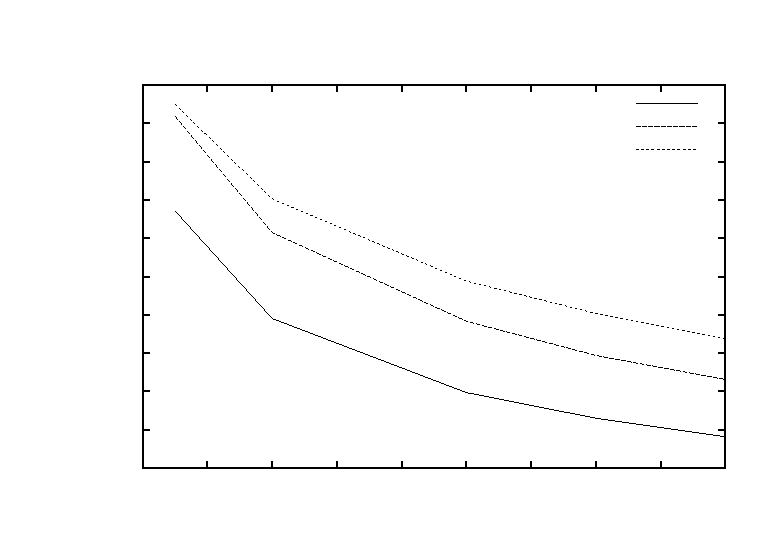
\includegraphics{chapters/chapter6/graphs/waste_robots}}%
    \gplfronttext
  \end{picture}%
\endgroup
}
\caption{Non-prioritized items over time over Swarm Density ($c$)}
\label{robotswasteplot}
\end{figure}

%Discussion
The purpose of examining the effect of additional robots is to determine whether the addition of extra robots negatively effects an algorithm's performance. An algorithm that would scale perfectly would show a linear increase in performance as the number of robots increases. The addition of more robots could potentially create interference between the robots or cause malfunction of the algorithms and impacting scalability. 

The hypothesis is that the honey bee algorithm would be the least impacted by the increase in swarm density since the robots will rest if they have not foraged an item for a particular period and thus the an increase in robots would not cause as much of an increase in interference. The na\"ive and desert ant algorithms should scale less effectively, since they have no mechanism to react to increased interference.

One needs to take care when selecting the environments for analysis. In order to confirm that any analysis about the slow down in the rate of foraging is caused by the increase in swarm density, one should only analyse environments where the robots are unable to complete foraging of all items for all robot densities. For this reason, the analysis has only been performed over a high object density where all items were not able to be foraged at any given swarm density where $S >= 200$ and $p >= 0.8$.

Table~\ref{specializationprioritized} and Figure~\ref{robotsgoldplot} indicate that the hypothesis is true as the honey bee is the most scalable since the addition of new robots negatively impacted the swarm the least, as in the rate of improvement as robots are added is closest to linear, however does slow down as swarm density gets very high indicating that the division of labour mechanism that allows an agent to switch to the waiting state when intereference is detected can likely be optimized. 

The na\"ive foraging algorithm improves very slowly as swarm density is increased indicated that adding more agents does not improve the algorithms performance very much. Since the na\"ive algorithm does not have any mechanism to react to increased interfence, these results are expected. The lack of such a machanism paired with the fact that the algorithm forages rather inefficiently to begin with likely means that the agents get stuck near the sink attempting to avoid each other and not managing to forage very much.

The desert ant algorithm is not as badly affected as the na\"ive algorithm by the increase in swarm density and is most likely a result of more optimal navigation allowing robots to stick to the paths they found instead of randomly navigating into one another. 

Examination of Table~\ref{specializationnonprioritized} and Figure~\ref{robotswasteplot} which show the effect of swarm density $c$ on $\mu$ are similar to those indicating the effect of swarm density $c$ on $\sigma$.

One can conclude that at least two factors effect the scalability of the swarm: the ability for the swarm to react to increased interference (like the honey bee algorithm) as well as the ability to avoid interference in the first place by having a more advanced navigation mechanism (like the desert ant algorithm).

\subsection{Environment Size}
\label{results:environmentsize}

%As environment size increases, how does the algorithm performance suffer

%Mann whitney U + average etc etc
%Graphs compareing performacne of # robots, per algorith, for each performance measure 2 performance measures

%NEED TABLES!!!!!!!!!

\begin{figure}[!htb]
\centering
\resizebox{\textwidth}{!}{% GNUPLOT: LaTeX picture with Postscript
\begingroup
  \makeatletter
  \providecommand\color[2][]{%
    \GenericError{(gnuplot) \space\space\space\@spaces}{%
      Package color not loaded in conjunction with
      terminal option `colourtext'%
    }{See the gnuplot documentation for explanation.%
    }{Either use 'blacktext' in gnuplot or load the package
      color.sty in LaTeX.}%
    \renewcommand\color[2][]{}%
  }%
  \providecommand\includegraphics[2][]{%
    \GenericError{(gnuplot) \space\space\space\@spaces}{%
      Package graphicx or graphics not loaded%
    }{See the gnuplot documentation for explanation.%
    }{The gnuplot epslatex terminal needs graphicx.sty or graphics.sty.}%
    \renewcommand\includegraphics[2][]{}%
  }%
  \providecommand\rotatebox[2]{#2}%
  \@ifundefined{ifGPcolor}{%
    \newif\ifGPcolor
    \GPcolorfalse
  }{}%
  \@ifundefined{ifGPblacktext}{%
    \newif\ifGPblacktext
    \GPblacktexttrue
  }{}%
  % define a \g@addto@macro without @ in the name:
  \let\gplgaddtomacro\g@addto@macro
  % define empty templates for all commands taking text:
  \gdef\gplbacktext{}%
  \gdef\gplfronttext{}%
  \makeatother
  \ifGPblacktext
    % no textcolor at all
    \def\colorrgb#1{}%
    \def\colorgray#1{}%
  \else
    % gray or color?
    \ifGPcolor
      \def\colorrgb#1{\color[rgb]{#1}}%
      \def\colorgray#1{\color[gray]{#1}}%
      \expandafter\def\csname LTw\endcsname{\color{white}}%
      \expandafter\def\csname LTb\endcsname{\color{black}}%
      \expandafter\def\csname LTa\endcsname{\color{black}}%
      \expandafter\def\csname LT0\endcsname{\color[rgb]{1,0,0}}%
      \expandafter\def\csname LT1\endcsname{\color[rgb]{0,1,0}}%
      \expandafter\def\csname LT2\endcsname{\color[rgb]{0,0,1}}%
      \expandafter\def\csname LT3\endcsname{\color[rgb]{1,0,1}}%
      \expandafter\def\csname LT4\endcsname{\color[rgb]{0,1,1}}%
      \expandafter\def\csname LT5\endcsname{\color[rgb]{1,1,0}}%
      \expandafter\def\csname LT6\endcsname{\color[rgb]{0,0,0}}%
      \expandafter\def\csname LT7\endcsname{\color[rgb]{1,0.3,0}}%
      \expandafter\def\csname LT8\endcsname{\color[rgb]{0.5,0.5,0.5}}%
    \else
      % gray
      \def\colorrgb#1{\color{black}}%
      \def\colorgray#1{\color[gray]{#1}}%
      \expandafter\def\csname LTw\endcsname{\color{white}}%
      \expandafter\def\csname LTb\endcsname{\color{black}}%
      \expandafter\def\csname LTa\endcsname{\color{black}}%
      \expandafter\def\csname LT0\endcsname{\color{black}}%
      \expandafter\def\csname LT1\endcsname{\color{black}}%
      \expandafter\def\csname LT2\endcsname{\color{black}}%
      \expandafter\def\csname LT3\endcsname{\color{black}}%
      \expandafter\def\csname LT4\endcsname{\color{black}}%
      \expandafter\def\csname LT5\endcsname{\color{black}}%
      \expandafter\def\csname LT6\endcsname{\color{black}}%
      \expandafter\def\csname LT7\endcsname{\color{black}}%
      \expandafter\def\csname LT8\endcsname{\color{black}}%
    \fi
  \fi
  \setlength{\unitlength}{0.0500bp}%
  \begin{picture}(7200.00,5040.00)%
    \gplgaddtomacro\gplbacktext{%
      \csname LTb\endcsname%
      \put(946,704){\makebox(0,0)[r]{\strut{} 0.1}}%
      \put(946,1112){\makebox(0,0)[r]{\strut{} 0.2}}%
      \put(946,1521){\makebox(0,0)[r]{\strut{} 0.3}}%
      \put(946,1929){\makebox(0,0)[r]{\strut{} 0.4}}%
      \put(946,2337){\makebox(0,0)[r]{\strut{} 0.5}}%
      \put(946,2746){\makebox(0,0)[r]{\strut{} 0.6}}%
      \put(946,3154){\makebox(0,0)[r]{\strut{} 0.7}}%
      \put(946,3562){\makebox(0,0)[r]{\strut{} 0.8}}%
      \put(946,3971){\makebox(0,0)[r]{\strut{} 0.9}}%
      \put(946,4379){\makebox(0,0)[r]{\strut{} 1}}%
      \put(1078,484){\makebox(0,0){\strut{} 50}}%
      \put(1714,484){\makebox(0,0){\strut{} 100}}%
      \put(2350,484){\makebox(0,0){\strut{} 150}}%
      \put(2986,484){\makebox(0,0){\strut{} 200}}%
      \put(3622,484){\makebox(0,0){\strut{} 250}}%
      \put(4259,484){\makebox(0,0){\strut{} 300}}%
      \put(4895,484){\makebox(0,0){\strut{} 350}}%
      \put(5531,484){\makebox(0,0){\strut{} 400}}%
      \put(6167,484){\makebox(0,0){\strut{} 450}}%
      \put(6803,484){\makebox(0,0){\strut{} 500}}%
      \put(176,2541){\rotatebox{-270}{\makebox(0,0){\strut{}Prioritized items over time ($\sigma$)}}}%
      \put(3940,154){\makebox(0,0){\strut{}Size ($S$)}}%
      \put(3940,4709){\makebox(0,0){\strut{}Prioritized items over time for each algorithm for different grid sizes}}%
    }%
    \gplgaddtomacro\gplfronttext{%
      \csname LTb\endcsname%
      \put(5816,4206){\makebox(0,0)[r]{\strut{}Na\"ive}}%
      \csname LTb\endcsname%
      \put(5816,3986){\makebox(0,0)[r]{\strut{}Desert Ant}}%
      \csname LTb\endcsname%
      \put(5816,3766){\makebox(0,0)[r]{\strut{}Honey Bee}}%
    }%
    \gplbacktext
    \put(0,0){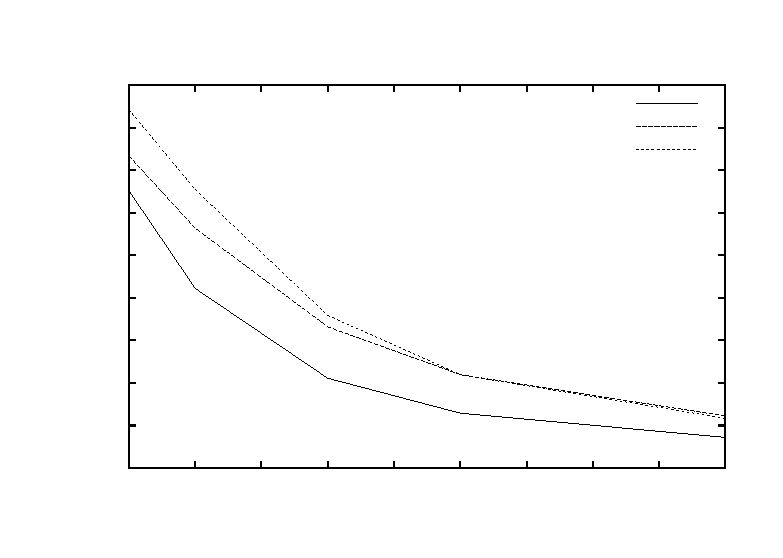
\includegraphics{chapters/chapter6/graphs/gold_sizes}}%
    \gplfronttext
  \end{picture}%
\endgroup
}
\caption{Environment Size}
\label{sizegoldplot}
\end{figure}

\begin{figure}[!htb]
\centering
\resizebox{\textwidth}{!}{% GNUPLOT: LaTeX picture with Postscript
\begingroup
  \makeatletter
  \providecommand\color[2][]{%
    \GenericError{(gnuplot) \space\space\space\@spaces}{%
      Package color not loaded in conjunction with
      terminal option `colourtext'%
    }{See the gnuplot documentation for explanation.%
    }{Either use 'blacktext' in gnuplot or load the package
      color.sty in LaTeX.}%
    \renewcommand\color[2][]{}%
  }%
  \providecommand\includegraphics[2][]{%
    \GenericError{(gnuplot) \space\space\space\@spaces}{%
      Package graphicx or graphics not loaded%
    }{See the gnuplot documentation for explanation.%
    }{The gnuplot epslatex terminal needs graphicx.sty or graphics.sty.}%
    \renewcommand\includegraphics[2][]{}%
  }%
  \providecommand\rotatebox[2]{#2}%
  \@ifundefined{ifGPcolor}{%
    \newif\ifGPcolor
    \GPcolorfalse
  }{}%
  \@ifundefined{ifGPblacktext}{%
    \newif\ifGPblacktext
    \GPblacktexttrue
  }{}%
  % define a \g@addto@macro without @ in the name:
  \let\gplgaddtomacro\g@addto@macro
  % define empty templates for all commands taking text:
  \gdef\gplbacktext{}%
  \gdef\gplfronttext{}%
  \makeatother
  \ifGPblacktext
    % no textcolor at all
    \def\colorrgb#1{}%
    \def\colorgray#1{}%
  \else
    % gray or color?
    \ifGPcolor
      \def\colorrgb#1{\color[rgb]{#1}}%
      \def\colorgray#1{\color[gray]{#1}}%
      \expandafter\def\csname LTw\endcsname{\color{white}}%
      \expandafter\def\csname LTb\endcsname{\color{black}}%
      \expandafter\def\csname LTa\endcsname{\color{black}}%
      \expandafter\def\csname LT0\endcsname{\color[rgb]{1,0,0}}%
      \expandafter\def\csname LT1\endcsname{\color[rgb]{0,1,0}}%
      \expandafter\def\csname LT2\endcsname{\color[rgb]{0,0,1}}%
      \expandafter\def\csname LT3\endcsname{\color[rgb]{1,0,1}}%
      \expandafter\def\csname LT4\endcsname{\color[rgb]{0,1,1}}%
      \expandafter\def\csname LT5\endcsname{\color[rgb]{1,1,0}}%
      \expandafter\def\csname LT6\endcsname{\color[rgb]{0,0,0}}%
      \expandafter\def\csname LT7\endcsname{\color[rgb]{1,0.3,0}}%
      \expandafter\def\csname LT8\endcsname{\color[rgb]{0.5,0.5,0.5}}%
    \else
      % gray
      \def\colorrgb#1{\color{black}}%
      \def\colorgray#1{\color[gray]{#1}}%
      \expandafter\def\csname LTw\endcsname{\color{white}}%
      \expandafter\def\csname LTb\endcsname{\color{black}}%
      \expandafter\def\csname LTa\endcsname{\color{black}}%
      \expandafter\def\csname LT0\endcsname{\color{black}}%
      \expandafter\def\csname LT1\endcsname{\color{black}}%
      \expandafter\def\csname LT2\endcsname{\color{black}}%
      \expandafter\def\csname LT3\endcsname{\color{black}}%
      \expandafter\def\csname LT4\endcsname{\color{black}}%
      \expandafter\def\csname LT5\endcsname{\color{black}}%
      \expandafter\def\csname LT6\endcsname{\color{black}}%
      \expandafter\def\csname LT7\endcsname{\color{black}}%
      \expandafter\def\csname LT8\endcsname{\color{black}}%
    \fi
  \fi
  \setlength{\unitlength}{0.0500bp}%
  \begin{picture}(7200.00,5040.00)%
    \gplgaddtomacro\gplbacktext{%
      \csname LTb\endcsname%
      \put(946,704){\makebox(0,0)[r]{\strut{} 0.1}}%
      \put(946,1112){\makebox(0,0)[r]{\strut{} 0.2}}%
      \put(946,1521){\makebox(0,0)[r]{\strut{} 0.3}}%
      \put(946,1929){\makebox(0,0)[r]{\strut{} 0.4}}%
      \put(946,2337){\makebox(0,0)[r]{\strut{} 0.5}}%
      \put(946,2746){\makebox(0,0)[r]{\strut{} 0.6}}%
      \put(946,3154){\makebox(0,0)[r]{\strut{} 0.7}}%
      \put(946,3562){\makebox(0,0)[r]{\strut{} 0.8}}%
      \put(946,3971){\makebox(0,0)[r]{\strut{} 0.9}}%
      \put(946,4379){\makebox(0,0)[r]{\strut{} 1}}%
      \put(1078,484){\makebox(0,0){\strut{} 50}}%
      \put(1714,484){\makebox(0,0){\strut{} 100}}%
      \put(2350,484){\makebox(0,0){\strut{} 150}}%
      \put(2986,484){\makebox(0,0){\strut{} 200}}%
      \put(3622,484){\makebox(0,0){\strut{} 250}}%
      \put(4259,484){\makebox(0,0){\strut{} 300}}%
      \put(4895,484){\makebox(0,0){\strut{} 350}}%
      \put(5531,484){\makebox(0,0){\strut{} 400}}%
      \put(6167,484){\makebox(0,0){\strut{} 450}}%
      \put(6803,484){\makebox(0,0){\strut{} 500}}%
      \put(176,2541){\rotatebox{-270}{\makebox(0,0){\strut{}Non-prioritized items over time ($\sigma$)}}}%
      \put(3940,154){\makebox(0,0){\strut{}Size ($S$)}}%
      \put(3940,4709){\makebox(0,0){\strut{}Non-prioritized items over time for each algorithm for different grid sizes}}%
    }%
    \gplgaddtomacro\gplfronttext{%
      \csname LTb\endcsname%
      \put(5816,4206){\makebox(0,0)[r]{\strut{}Na\"ive}}%
      \csname LTb\endcsname%
      \put(5816,3986){\makebox(0,0)[r]{\strut{}Desert Ant}}%
      \csname LTb\endcsname%
      \put(5816,3766){\makebox(0,0)[r]{\strut{}Honey Bee}}%
    }%
    \gplbacktext
    \put(0,0){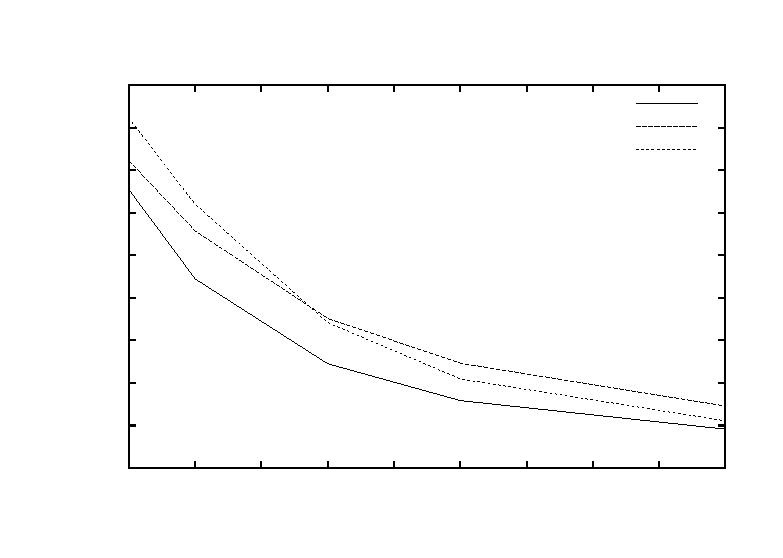
\includegraphics{chapters/chapter6/graphs/waste_sizes}}%
    \gplfronttext
  \end{picture}%
\endgroup
}
\caption{Non-prioritized items over time for different environment sizes for each algorithm}
\label{sizewasteplot}
\end{figure}

As the environment size increases, one would expect the performance to get quadratically less since the algorithms were run for the same amount of time. For this analysis, the experiments would ideally be run until no more items can be foraged, but due to time constraints only a limited study could be performed. For this reasons, the results have been presented however no valid analysis can be performed.

\section{Summary}
\label{results:summary}

This chapter presented the results of the experiments and performed a detailed analysis. The results were discussed around three axes: flexibility, robustness and scalability. An overview of the results seems to show that the honey bee algorithm performed the best over all environments and initial swarm configurations, while the desert ant performed next best and lastly followed by the na\"ive algorithm. 

Flexibility addressed how the algorithms cope with differing types of distributions of prioritized and nonprioritized items that concluded that the honey bee algorithm performs less effectively on the simpler environments (vein and gaussian environments) since the simpler environments lead the division of labour mechanism to incorrectly detect a change rich areas of prioritized items and thus are negatively impacted by the overhead of division of labour. Flexibility also addressed the dependancy between various environment item ratios $r$ compared to specialization ratio $\tau$ of the na\"ive and desert ant algorithms and the independance of the honey bee algorithm on $r$ and $\tau$ due to the division of labour on a specialization level. 

Robustness can be defined as an algorithms ability to degrade gracefully or recover from damage or malfunction to of a portion of the swarm and was analysed in terms of the algorithms' dependance on the initial swarm specialization ratio $\tau$. It was determined that the honey bee algorithm is superior in robustness since the performance of the swarm is independant of $\tau$ and thus if a portion of the prioritized item foraging swarm is damaged, the specialization division of labour mechanism of the honey bee algorithm allows robots foraging non-prioritized items to switch to foraging prioritized items when needed.

Lastly, scalability is discussed in terms of whether an increase in swarm density $c$ (ie the number of robots in the swarm) will result in increased robot-to-robot interference and thus a less effective swarm. It was determined that both an algorithm that can firstly avoid interference by using more advanced navigation and avoidance of other robots (as indicated by the desert ants) as well as by the swarm reacting to an increase in interference by placing a portion of the swarm into a rest state in times of high interference. Despite showing signs of a slowing in improvement as swarm density increased beyond a certain point, the honey bee algorithm had the ability to react to interference, likely due to the bee-like foraging division of labour that allows robots to rest and conserve energy when the stage is too busy and interference is resulting in failed foraging trips. The na\"ive algorithm reacted very badly to an increase in swarm density and the desert ant performed better than the na\"ive algorithm 

%%%%%%%%%%%%%%%%%%%%%%%%%%%%%%%%%%%%%%%%%%%%%%%%%
%%%%%%%%%%%%%%%%%%%%%%%%%%%%%%%%%%%%%%%%%%%%%%%%%